%%%%%%%% ICML 2026 EXAMPLE LATEX SUBMISSION FILE %%%%%%%%%%%%%%%%%

\documentclass{article}

% Recommended, but optional, packages for figures and better typesetting:
\usepackage{microtype}
\usepackage{graphicx}
\usepackage{subcaption}
\usepackage{booktabs} % for professional tables

% hyperref makes hyperlinks in the resulting PDF.
% If your build breaks (sometimes temporarily if a hyperlink spans a page)
% please comment out the following usepackage line and replace
% \usepackage{icml2026} with \usepackage[nohyperref]{icml2026} above.
\usepackage{hyperref}


% Attempt to make hyperref and algorithmic work together better:
\newcommand{\theHalgorithm}{\arabic{algorithm}}
\usepackage{algorithm}
\usepackage{algorithmic}
% Use the following line for the initial blind version submitted for review:
%\usepackage{icml2026}

% For preprint, use
\usepackage[preprint]{icml2026}

% If accepted, instead use the following line for the camera-ready submission:
% \usepackage[accepted]{icml2026}

\usepackage{amsmath}
\usepackage{amssymb}
\usepackage{mathtools}
\usepackage{amsthm}
\usepackage{multirow}
\usepackage{booktabs}
\usepackage{makecell}
\usepackage{array}
\usepackage{arydshln} % 导言区加入
\usepackage{tabularx}




% if you use cleveref..
\usepackage[capitalize,noabbrev]{cleveref}

%%%%%%%%%%%%%%%%%%%%%%%%%%%%%%%%
% THEOREMS
%%%%%%%%%%%%%%%%%%%%%%%%%%%%%%%%
\theoremstyle{plain}
\newtheorem{theorem}{Theorem}[section]
\newtheorem{proposition}[theorem]{Proposition}
\newtheorem{lemma}[theorem]{Lemma}
\newtheorem{corollary}[theorem]{Corollary}
\theoremstyle{definition}
\newtheorem{definition}[theorem]{Definition}
\newtheorem{assumption}[theorem]{Assumption}
\theoremstyle{remark}
\newtheorem{remark}[theorem]{Remark}

\newcommand{\method}{DualSpec}

% Todonotes is useful during development; simply uncomment the next line
%    and comment out the line below the next line to turn off comments
%\usepackage[disable,textsize=tiny]{todonotes}
\usepackage[textsize=tiny]{todonotes}

% The \icmltitle you define below is probably too long as a header.
% Therefore, a short form for the running title is supplied here:
\icmltitlerunning{DualSpec: Accelerating Deep Research Agents
via Dual-Process Action Speculation}

\begin{document}

\twocolumn[
  \icmltitle{DualSpec: Accelerating Deep Research Agents\\ via Dual-Process Action Speculation}

  % It is OKAY to include author information, even for blind submissions: the
  % style file will automatically remove it for you unless you've provided
  % the [accepted] option to the icml2026 package.

  % List of affiliations: The first argument should be a (short) identifier you
  % will use later to specify author affiliations Academic affiliations
  % should list Department, University, City, Region, Country Industry
  % affiliations should list Company, City, Region, Country

  % You can specify symbols, otherwise they are numbered in order. Ideally, you
  % should not use this facility. Affiliations will be numbered in order of
  % appearance and this is the preferred way.
  \icmlsetsymbol{equal}{*}
  \icmlsetsymbol{intern}{$\dagger$}

  \begin{icmlauthorlist}
    \icmlauthor{Shuzhang Zhong}{pku,intern}
    \icmlauthor{Baotong Lu}{msr,equal}
    \icmlauthor{Qi Chen}{msr}
    \icmlauthor{Chuanjie Liu}{ms}
    \icmlauthor{Fan Yang}{msr}
    \icmlauthor{Meng Li}{pku,equal}
  \end{icmlauthorlist}

  \icmlaffiliation{pku}{Peking University, Beijing, China}
  \icmlaffiliation{msr}{Microsoft Research}
  \icmlaffiliation{ms}{Microsoft}

  \icmlcorrespondingauthor{Baotong Lu}{baotonglu@microsoft.com}
  \icmlcorrespondingauthor{Meng Li}{meng.li@pku.edu.cn}
 

  % You may provide any keywords that you find helpful for describing your
  % paper; these are used to populate the "keywords" metadata in the PDF but
  % will not be shown in the document
  \icmlkeywords{Machine Learning, ICML}

  \vskip 0.3in
]

% this must go after the closing bracket ] following \twocolumn[ ...

% This command actually creates the footnote in the first column listing the
% affiliations and the copyright notice. The command takes one argument, which
% is text to display at the start of the footnote. The \icmlEqualContribution
% command is standard text for equal contribution. Remove it (just {}) if you
% do not need this facility.

% Use ONE of the following lines. DO NOT remove the command.
% If you have no special notice, KEEP empty braces:
\printAffiliationsAndNotice{$\dagger$Work performed during the internship while at Microsoft Research.} % no special notice (required even if empty)
% Or, if applicable, use the standard equal contribution text:
% \printAffiliationsAndNotice{\icmlEqualContribution}

\begin{abstract}

% Large language model based deep research agents have been increasingly popular to address open-ended, long-horizon information-seeking tasks.
% However, they often suffer from high end-to-end latency due to extensive reasoning and frequent tool use. 
% Speculation frameworks overlap action execution with reasoning to reduce latency, yet existing methods rely on uniform speculation and strict action matching, limiting both inference speedups and robustness.

% In this work, we revisit the speculate–verify scheme for deep research agents through the lens of action heterogeneity.
% We observe that Search and Visit require fundamentally different reasoning and model capacity demands: our entropy-based analysis shows that Search has higher decision entropy and benefits more from reasoning, while Visit has lower entropy and depends more on model capacity.
% Motivated by this dual-process property, we propose \method{}, a heterogeneous speculation framework with a lightweight confidence-based semantic verifier.
% Experiments across models and benchmarks show that \method{} achieves up to 3.28$\times$ speedup while maintaining accuracy comparable to full-reasoning agents.


Large language model-based deep research agents have been increasingly popular for addressing long-horizon information-seeking tasks, but they often incur high end-to-end latency due to extensive reasoning and frequent tool use. Speculation frameworks aim to reduce latency by overlapping action execution with reasoning; however, existing approaches typically rely on uniform speculation strategies and strict action matching, which limits inference speedups and robustness.

In this work, we revisit the speculate-verify paradigm for deep research agents through the lens of action heterogeneity. We show that \textit{Search} and \textit{Visit} actions exhibit fundamentally different reasoning and model capacity requirements: entropy-based analysis reveals that Search decisions have higher uncertainty and benefit significantly from explicit reasoning, whereas Visit decisions have lower entropy and depend primarily on model capacity. Motivated by this dual-process characteristic, we propose \method{}, a heterogeneous speculation framework equipped with a lightweight, confidence-based semantic verifier. Experiments across multiple models and benchmarks demonstrate that \method{} achieves up to 3.28$\times$ end-to-end speedup while maintaining accuracy comparable to fully reasoning agents.



 
\end{abstract}

%\input{docs/outline}

\section{Introduction}

\iffalse
Outline: 
1. LLM reasoning capacity => external tools => agents; Deep research agent is important and popular
2. High performance comes at time efficiency: (1) extensive token costs for reasoning (2) sequential nature of 
mutli-turn reasoning-action-observation. Should we have a profiling of reasoning time and functional call time?
    - It typically requires a strong model with high parameter capacity and long reasoning 
3. latency is very critical for users, especially deep research agents. 
4. Corroborating with recent works, we find that action is the right barrier for speculation and verification 
5. However, how to speculative and how to verify to balance the accuracy and efficiency is challenging 
   - How to improve the accuracy of speculation => thus the verification pass rate higher => higher efficiency
   - How to verify smartly, to ensure the agent performance is not compromised 
6. Our observation: different actions require different speculation strategies for the agent to be efficient and accurate
   - Search action: high uncertainty, underspecified query => need strong reasoning to reduce the uncertainty => smaller model with reasoning 
   - Visit action: low uncertainty, concrete content => strong parametric prior is more important => large model without reasoning 
   - This is aligned with system 1 and system 2 thinking in cognitive science 
   - We prove this with entropy analysis of different actions and end-to-end experiments
7. Our framework: Heterogeneous speculation framework for deep research agents 
   - Draft model: smaller model with reasoning for system 2 action; large model without reasoning for system 1 action
   - verification model: large model judge
8. Evaluation results
8. Contributions

Outline
1. In this work, we rethink the speculate-verify paradigm for deep research agents by carefully analyzing action heterogeneity and verification trade-offs.

2. Our goal is to improve the accuracy of action speculation to improve the acceptance ratio and thus enhance the efficiency, while designing effective verification to maintain the agent performance.

3. We observe that, to predict next action more accurately, different actions require different speculation strategies based on their distinct characteristics and demands.
    - Deep research agents mainly involve two types of actions: Search and Visit, where a search action issue a query to the search engine to retrieve relevant webpages (URL lists), while a visit action access a specific webpage to extract its content.
    - We find that generating a high-quality Search action demands strong reasoning capabilities to reduce the inherent uncertainty in query formulation, while Visit actions benefit more from robust parametric knowledge and less from explicit reasoning because it only requires choose one specific URL from a concrete list, with less action space. 
    - We confirms this with an entropy-based analysis of action decisions and end-to-end studies.
    - This is similar to the cognitive science distinction between \textit{System 2} (deliberative) and \textit{System 1} (intuitive) decision making, where search aligns with System 2 behavior and visit with System 1 behavior.
    - There are typically two lightweight speculation methods: small model with reasoning and large model which directly generates actions without reasoning.
    - According to the above property, using a small model with reasoning to draft search action and a large model without reasoning to draft visit action can yield higher speculation accuracy.

4. The verification design should be also carefully considered to ensure high efficiency and the agent performance is not compromised. Do the exact action match is too strict because two queries generated by different models can be semantically similar but not exactly the same. Moreover, do the action match requires the base model to first finish its reasoning, which can be time-consuming and delay the verification process. 

Given the above observations and challenges, we propose \method, a heterogeneous action speculation framework for deep research agents.

- Our method: the critical path does not have base model reasoning
\fi

% The increasing reasoning capabilities of Large Language Models (LLMs) enables them to interact with external tools and environments, facilitating the development of intelligent agents~\cite{yao2022react,shinn2023reflexion}.
% Notably, deep research agents have emerged as a prominent application to solve open-ended, long-horizon research tasks with high information-seeking and reasoning demands~\cite{deepresearch}.  
% Through the multi-step reasoning and tool-use paradigm, these agents continuously gather evidence from external resources such as search engines and refine hypotheses iteratively, moving beyond static question answering to tackling complex research problems. 

The increasing reasoning capabilities of large language models (LLMs) enable interaction with external tools and environments, driving the development of intelligent agents~\cite{yao2022react,shinn2023reflexion,schick2023toolformer}.
Among these, deep research agents have emerged as a prominent application for addressing open-ended, long-horizon research tasks with high information-seeking and reasoning demands~\cite{deepresearch}.
By iteratively reasoning and invoking external tools such as search engines, these agents accumulate evidence and refine hypotheses, extending beyond static question answering to complex research problems.

\begin{figure}
    \centering
    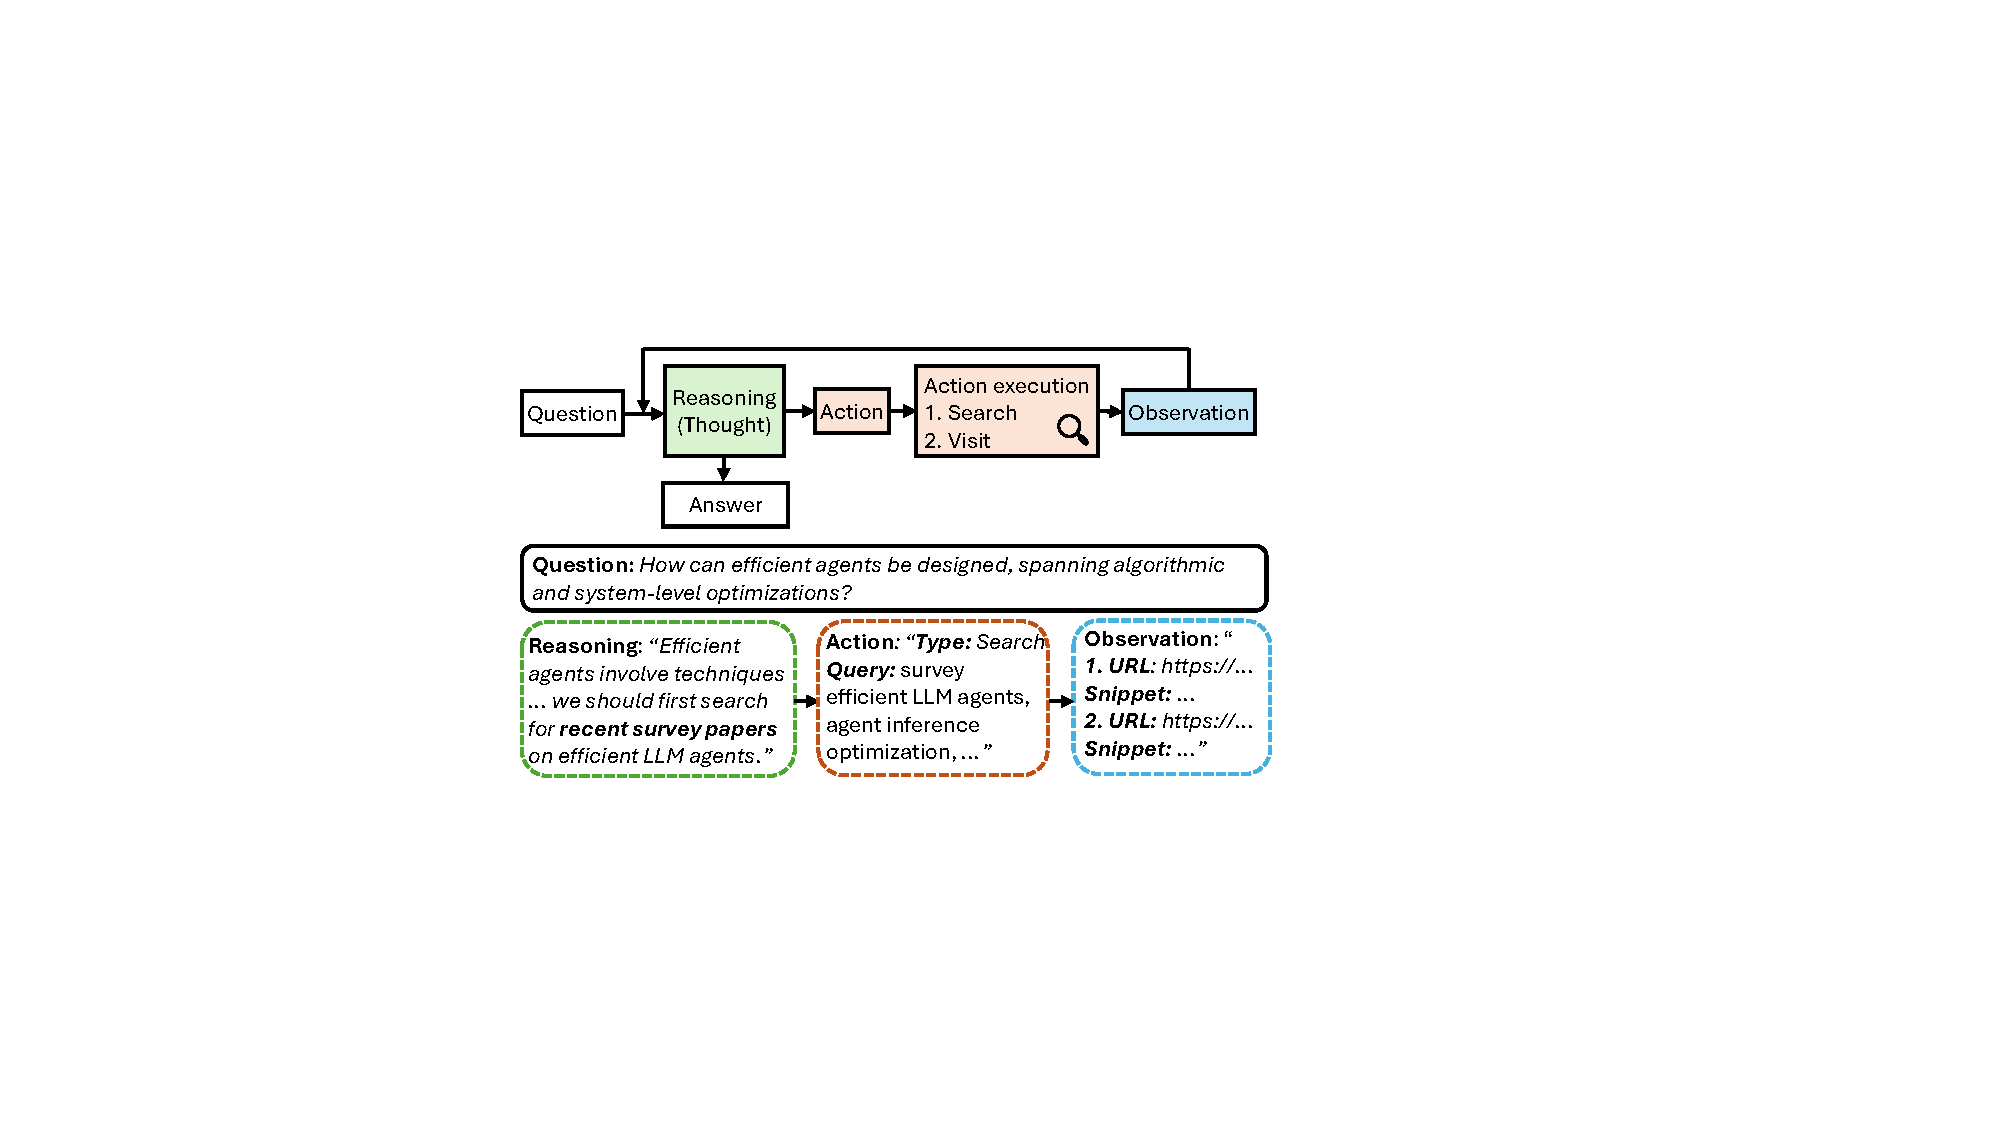
\includegraphics[width=\linewidth]{figs/deep_research.pdf}
    \caption{Deep research agent workflow. Deep research agents follow a Reason-Action-Observation loop, where the agent alternates between generating reasoning traces and executing actions (Search or Visit) to gather information.}
    \label{fig:deep_research}
\end{figure}


% Despite its advancements, deep research agents often suffer from high inference latency.
% As shown in Figure~\ref{fig:deep_research}, LLM agent often follows the Reason-Action (ReAct) paradigm \cite{yao2022react} with 
% a strict sequential dependency: the model must synthesize a complete reasoning trace 
% before emitting an executable action and then, wait for the subsequent observations before moving forward to the next reasoning phase. 
% Both the reasoning process and the action execution can be time-consuming, especially when the agent relies on large models with extensive token usage for reasoning and interacts with external tools that may have variable response times.
% The reasoning-action-observation cycle repeats for multiple turns until the agent reaches a final answer, 
% often requiring minutes, if not hours, to answer a single query. 

Despite their effectiveness, deep research agents often incur high inference latency.
As shown in Figure~\ref{fig:deep_research}, agents typically follow the ReAct paradigm~\cite{yao2022react} with strict sequential dependencies: the model must complete a reasoning trace before emitting an action and then wait for the resulting observation before proceeding.
Both reasoning and action execution can be time-consuming, particularly when using large models with long reasoning traces and external tools with variable response times\cite{kim2023llm,zhang2025optimizing}.
This reasoning--action--observation cycle repeats over many turns until a final answer is produced, often requiring minutes or longer for a single query.


% To mitigate this inefficiency, a promising direction is to leverage the speculate-verify paradigm, in which a lightweight model or strategy speculates the next action and executes it immediately, while the base model concurrently performs its reasoning process~\cite{huang2025reducing,guan2025dynamic}.
% If the base model generates an action consistent with the speculative one, 
% it skips the action execution and directly accept the speculative tool call response (observation), saving the latency; when they disagree, the base model executes as usual.
% This paradigm differs from, and complements, speculative decoding~\cite{leviathan2023fast}, as it operates at the level of agent actions rather than language tokens, enabling latency reduction through parallelism between reasoning and tool use.
% However, a fundamental challenge lies in how to design effective speculation and verification strategies that balance the agent efficiency and accuracy.
% Inaccurate next-action prediction or conservative verification can lead to frequent fallbacks to the base model, diminishing efficiency gains, while overly permissive verification risks degrading the agent's overall performance.

A promising approach to reduce latency is the speculate--verify paradigm, where a lightweight model or strategy speculates the next action and executes it immediately, while the base model concurrently performs its reasoning~\cite{huang2025reducing,guan2025dynamic}.
If the base model's action matches the speculative one, the speculative observation is directly accepted, saving execution time; otherwise, the base model executes the action as usual.
Unlike speculative decoding~\cite{leviathan2023fast}, this approach operates at the action level rather than the token level, enabling parallelism between reasoning and tool use.
However, designing effective speculation and verification remains challenging: inaccurate speculation or conservative verification leads to frequent fallbacks and limited speedups, whereas overly permissive verification risks degrading agent performance.


% In this work, we rethink the speculate--verify paradigm for deep research agents through a principled analysis of action heterogeneity and verification trade-offs.
% The lightweight speculation approaches typically fall into two categories: (i) small models with explicit reasoning, and (ii) large models that directly emit actions without reasoning.
% We observe that different action types exhibit markedly different uncertainty profiles and thus call for distinct speculation strategies.
% In particular, deep research agents predominantly rely on two actions: Search and Visit.
% A Search action formulates a query to retrieve a list of relevant webpages, whereas a Visit action selects and accesses a specific URL from the candidate set.
% We find that generating effective Search actions requires strong reasoning to resolve high uncertainty in query formulation, while Visit actions operate over a much more constrained action space and rely primarily on parametric knowledge, with limited need for explicit reasoning.


In this work, we rethink speculate--verify for deep research agents through a principled analysis of action heterogeneity and verification trade-offs.
Existing lightweight speculation methods generally adopt either (i) small models with explicit reasoning or (ii) large models that emit actions without reasoning.
We observe that different action types exhibit distinct uncertainty profiles and thus require different speculation strategies.
Deep research agents primarily use two actions: \textit{Search}, which formulates a query to retrieve relevant webpages, and \textit{Visit}, which selects and accesses a specific URL from a candidate set.
Search involves high uncertainty in query formulation and benefits from strong reasoning, whereas Visit operates over a constrained action space and relies mainly on parametric knowledge.


% We substantiate this distinction through an entropy-based analysis of action decision-making with and without reasoning, complemented by end-to-end empirical studies.
% Our results consistently show that Search actions exhibit higher uncertainty than Visit actions, and explicit reasoning helps reduce uncertainty for Search but yields marginal benefits for Visit.
% This finding closely mirrors the cognitive science dichotomy between \textit{System~2} (deliberative) and \textit{System~1} (intuitive) thinking mode, with Search aligning with the former and Visit with the latter.
% Motivated by these insights, we show that aligning speculation mechanisms with action characteristics -- using a small reasoning model for Search and a large model without explicit reasoning for Visit -- significantly improves speculation accuracy.

We validate this distinction via end-to-end empirical evaluations, together with an entropy-based analysis of action decisions with and without reasoning.
Across settings, Search actions exhibit much higher uncertainty than Visit actions; explicit reasoning helps reduce uncertainty for Search but provides marginal gains for Visit.
This pattern aligns with the cognitive science distinction between \textit{System~2} (deliberative) and \textit{System~1} (intuitive) reasoning, with Search corresponding to the former and Visit to the latter.
Guided by these insights, we show that matching speculation strategies to action characteristics -- using a small reasoning model for Search and a large model without reasoning for Visit -- significantly improves speculation accuracy.

% Beyond speculation, verification also plays an critical role in achieving high efficiency without sacrificing agent performance.
% Exact action matching is often overly restrictive: two actions may be semantically equivalent despite token-level differences, especially for Search queries.
% Moreover, action-based verification -- whether exact or approximate -- typically requires the base model to complete its full reasoning process before verification can occur, placing reasoning on the critical path and limiting potential latency reductions.

Verification is also critical for achieving efficiency without sacrificing performance.
Exact action matching is often overly restrictive, as semantically equivalent actions, especially queries, may differ at the token level.
Moreover, action-based verification typically requires the base model to complete reasoning before verification, placing reasoning on the critical path and limiting latency reductions.


% Based on these observations, we propose \method, a heterogeneous action speculation framework for deep research agents that tailors speculation and verification to action-specific properties.
% \method~employs a small reasoning model to speculate actions, while allowing the large base model to concurrently generate a Visit action without explicit reasoning.
% If the speculative action is Search, the agent adopts the small model's output as the draft; otherwise, it uses the base model's directly generated Visit action.
% For verification, rather than performing explicit action matching, \method~leverages the base model's internal confidence to determine whether to accept the drafted action, thereby removing the base model's reasoning from the critical path.

Based on these observations, we propose \method, a heterogeneous action speculation framework for deep research agents that tailors speculation and verification to action-specific properties.
\method~uses a small reasoning model to speculate actions, while allowing the base model to concurrently generate a Visit action by skipping reasoning.
It dynamically selects an appropriate draft based on the reasoning state.
For verification, \method~leverages the base model's internal confidence rather than explicit action matching, removing base-model reasoning from the critical path while preserving the agent performance.

% We implement \method~and evaluate its accuracy and efficiency on two representative reasoning models, MiroThinker~\cite{team2025mirothinker} and Qwen-3~\cite{team2025tongyi}, using widely used deep research benchmarks, including GAIA-Text-103~\cite{wu2025webdancer}, XBench\_DeepSearch~\cite{chen2025xbench} and Seal-0~\cite{pham2025sealqa}.
% Our results show that \method~achieves up to \textbf{3.28}$\times$ end-to-end latency speedup while maintaining performance comparable to the base model with full reasoning.

We implement \method~and evaluate it on two representative reasoning models, MiroThinker~\cite{team2025mirothinker} and Qwen-3~\cite{team2025tongyi}, using popular deep research benchmarks including GAIA-Text-103~\cite{wu2025webdancer}, XBench-DeepSearch~\cite{chen2025xbench}, and Seal-0~\cite{pham2025sealqa}.
\method~achieves up to \textbf{3.28}$\times$ end-to-end latency speedup while maintaining performance comparable to the fully reasoning base model.





\iffalse
Initial draft:

Recent advances in Large Language Models (LLMs) have given rise to deep research agents. These agents can perform multi-step reasoning and seeking information across the internet, allowing them to gather evidence and iteratively refine intermediate hypotheses\cite{team2025mirothinker,team2025tongyi}.
This iterative process of reasoning and interaction allows agents to move beyond static question answering and address increasingly complex, long-horizon research tasks.

However, the advancements of deep research agents often incur a substantial latency overhead. This bottleneck can be derived from the Reason–Action (ReAct) paradigm\cite{yao2022react}, which enforces a strict sequential dependency: the model must synthesize a complete reasoning trace before emitting an executable action and awaiting the subsequent observation. As a result, the agent cannot begin interacting with the environment until it has fully completed its internal reasoning for the current step.

To mitigate this inefficiency, recent works have proposed a range of latency-oriented optimizations. 
A common strategy is to leverage lightweight inference methods for most steps, while selectively invoking original reasoning only when needed\cite{guan2025dynamic}. Such lightweight approaches include delegating inference to smaller or quantized models\cite{bian2025limits}, or skipping the reasoning process entirely\cite{huang2025reducing}.

Despite their effectiveness, existing approaches largely adopt a homogeneous view of agent actions and apply a uniform lightweight strategy across all actions. They use a same lightweight method for all of the actions. Such designs often yield inaccurate or underpowered decisions, proving ineffective in practice by either triggering frequent fallback to high-capacity models or resulting in longer exploration trajectories \cite{lin2025towards}.

In this work, we make a simple yet underexplored observation: deep research agents involve two types of actions, Search and Visit. A Search action issues queries to search engines (e.g., Google or Bing) to retrieve relevant webpages. A Visit action accesses webpages or local files and extracts or summarizes their content. Search actions require the agent to translate underspecified goals into effective queries. This process typically demands explicit reasoning and exhibits high uncertainty.
In contrast, Visit actions operate on concrete retrieved content, involving localized decisions such as selecting, filtering, or extracting relevant information, which tend to be more deterministic and rely primarily on parametric knowledge.

This asymmetry mirrors a well-established distinction between deliberative and intuitive decision making.
From the perspective of \textit{System 2} versus \textit{System 1}, Search aligns with \textbf{System 2} behavior, emphasizing \textbf{reasoning depth} over model scale, whereas Visit corresponds to \textbf{System 1} behavior, relying primarily on \textbf{parametric capacity} rather than explicit logical reasoning.
 
Motivated by this observation, we propose \method, a collaboration framework that generates System 1 and System 2 actions heterogeneously based on their different inference demands. Rather than uniformly using the same lightweight method, \method dynamically assigns deliberative reasoning with smaller model to cognitively demanding System 2 actions, while executing System 1 actions using the origin full-size model but without the reasoning process.
Our contributions can be summarized as follows:

\begin{itemize}
    \item We identify a fundamental action-level asymmetry in deep research agents by analyzing the entropy of action decisions. We show that \textit{System 2} actions (e.g., Search) exhibit high initial uncertainty, where explicit reasoning plays a critical role in reducing action entropy, whereas \textit{System 1} actions (e.g., Visit) naturally operate in low-entropy regimes and gain little from reasoning, instead benefiting from strong parametric priors.
    
    \item We propose \method, a heterogeneous collaboration framework that decouples \textit{System 2} and \textit{System 1} actions in agent execution. \method assigns a smaller model with explicit reasoning to handle \textit{System 2} actions, while using the original full-size model to directly generate \textit{System 1} actions without reasoning, and selectively escalates to full reasoning with the large model when necessary.
    
    \item We implement the \method  on top of MiroThinker and SGLang and demonstrate up to $xxx\times$ speedup over prior-art collaboration frameworks without compromising accuracy.
\end{itemize}
\fi
\section{Background and Related Work}

\subsection{Deep Research Agents}
% Deep research agents address long-horizon, open-ended information-seeking tasks by iteratively reasoning and interacting with external tools such as search engines and web browsers. 
Given an input question, deep research agents operate in a multi-step loop that alternates between reasoning to generate an action, executing the tool call, and incorporating the response into its context, until producing a final answer~\cite{zhang2025agentorchestra,huang2025deep}.


\begin{figure}
\centering
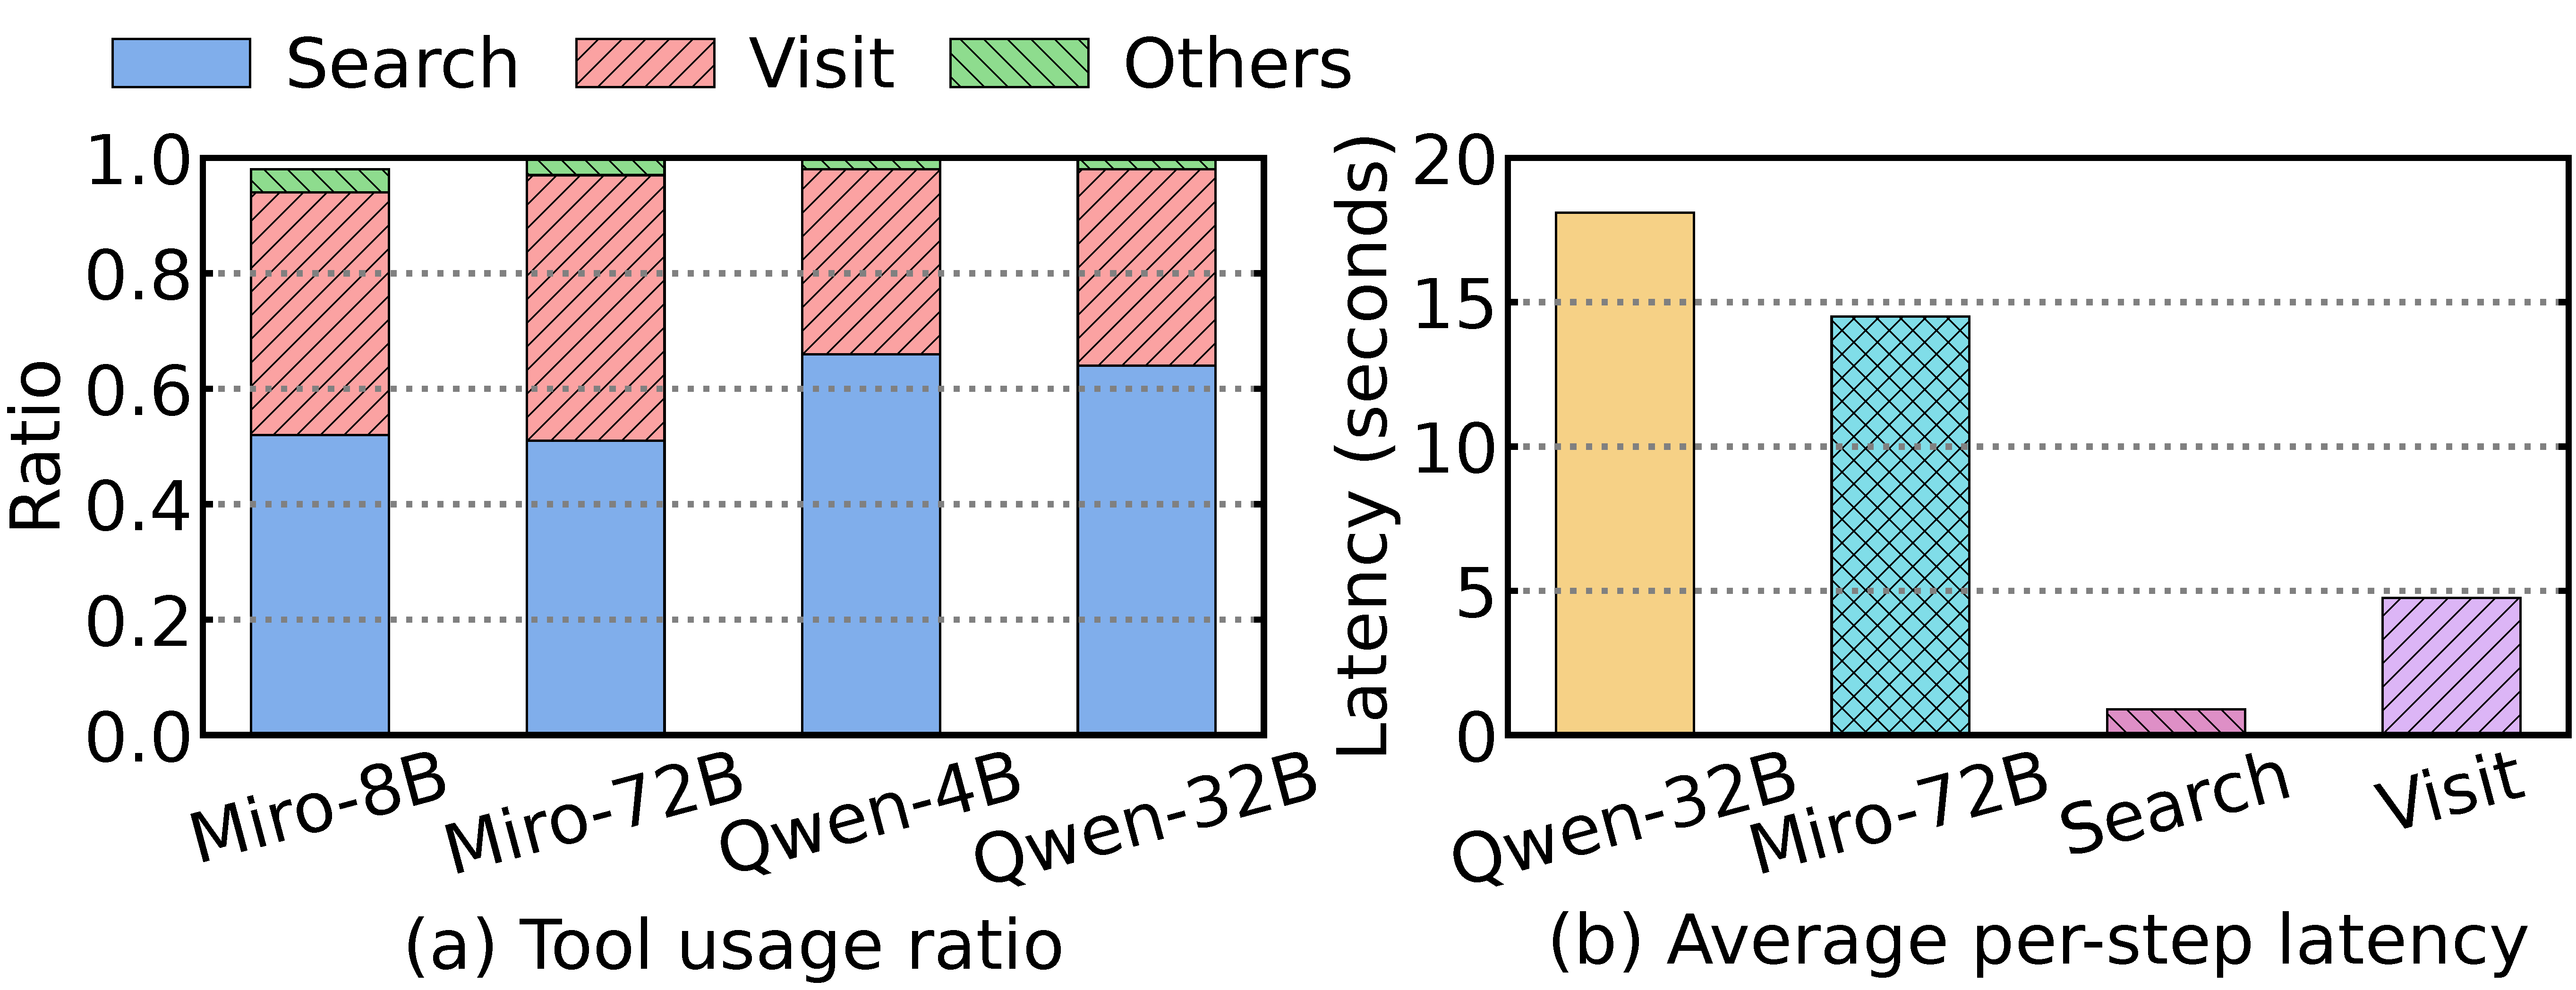
\includegraphics[width=\linewidth]{figs/draw_basics.pdf}
\caption{
Deep research inference characteristics using different models. ``Miro'' denotes ``MiroThinker'' while 
``Qwen'' denotes ``Qwen-3''.     
(a) Tool usage ratio on the GAIA benchmark\footnotemark. (b) Time breakdown per step on model reasoning and tool execution. Model reasoning accounts for a significant fraction of the total latency.}
\label{fig:action_ratio}
\end{figure}

\footnotetext{Unless otherwise specified, all micro-level analyses are conducted on the GAIA benchmark; consistent trends are observed across other benchmarks.}

% Most deep research agents rely on two core actions in their workflows: \textit{Search} and \textit{Visit}. 
% The \textit{Search} action formulates a query to retrieve a list of candidate webpages, each 
% accompanied by a brief snippet. 
% The \textit{Visit} action then selects a specific URL and provides a concise instruction 
% specifying what information to extract from the page. 
% To execute these actions, \textit{Search} directly interacts with a search engine, 
% whereas \textit{Visit} accesses the selected webpage and typically invokes an LLM to summarize 
% task-relevant content according to the instruction. 
% This design helps filter out irrelevant information and limits unnecessary context growth in the agent. 
% Figure~\ref{fig:action_ratio}(a) reports 
% the relative frequency of these actions when running tasks on the GAIA benchmark.  
% The results demonstrate that they are used at comparable rates, with \textit{Search} occurring slightly 
% more often due to query reformulation when retrieved results are unsatisfactory.
% Other tool calls (e.g., code execution) account for only a small fraction of steps.

Most deep research agents rely on two core actions: Search and Visit.
Search consists of a query used to retrieve candidate webpages with brief snippets, while Visit selects a URL and specifies an instruction for extracting relevant information.
During execution,
Search directly queries a search engine, whereas Visit accesses the webpage and typically invokes an LLM to summarize task-relevant content according to the instruction\cite{nakano2021webgpt, zhou2023webarena}.
This design filters irrelevant information and limits unnecessary context growth.
Figure~\ref{fig:action_ratio}(a) shows that these actions occur at comparable frequencies, with Search used slightly more often due to query reformulation when results are unsatisfactory.
Other tool calls (e.g., code execution) constitute only a small fraction of steps.


% Despite strong problem-solving capabilities, deep research agents often incur high latency due to the multi-step nature of their reasoning and tool-use workflows. We measure the per-step time breakdown by running the agent on the A100 GPU and show the results Figure~\ref{fig:action_ratio}(b). Model reasoning constitutes a significant portion of the total latency, while tool execution introduces additional, though smaller, delays. When accumulated over many iterations, these costs lead to long end-to-end response times, hindering user experience and practical deployment. 

Despite strong problem-solving performance, deep research agents often incur high latency due to their multi-step reasoning and tool-use workflows.
Figure~\ref{fig:action_ratio}(b) reports the per-step time breakdown measured on the A100 GPU.
Model reasoning dominates total latency, while tool execution introduces additional, though smaller, overheads.
Accumulated over many iterations, these costs lead to long end-to-end response times, limiting usability and deployment.

\subsection{Agent Optimization}

% Stronger backbone models and richer interactions with external tools improve agent performance on challenging tasks~\cite{yao2022react}.
% However, these gains often come at the cost of time efficiency, as longer reasoning traces and more frequent tool interactions lead to increased latency. 
% Recent studies observe that not all agent steps are equally challenging~\cite{zhang2023ecoassistant,saha2024system}. 
% This insight motivates optimization techniques that offload simpler steps to lightweight models while reserving more complex reasoning for stronger models, thereby balancing performance and efficiency.

Stronger backbone models and richer tool interactions improve agent performance on challenging tasks~\cite{shang2025rstar2}, but often reduce time efficiency due to longer reasoning traces and more frequent tool use.
Recent work observes that agent steps vary in difficulty~\cite{zhang2023ecoassistant,saha2024system}, motivating approaches that delegate simpler steps to lightweight models while reserving complex reasoning for stronger models.

% In this context, speculate--verify paradigms have emerged as a promising direction for reducing agent latency~\cite{ye2025speculative,guan2025dynamic,hua2024interactive,wang2025accelerating}. 
% Dynamic Speculative Planning~\cite{guan2025dynamic} introduces a lightweight speculator (e.g., a small reasoning model) to draft an action and obtain its result, while a stronger base model concurrently performs full reasoning. 
% The speculative action is verified against the base model action using criteria such as minimum edit distance, and the speculative tool call response is reused when they agree, reducing overall latency. 
% SPAgent~\cite{huang2025reducing} skips explicit reasoning in early stages to generate actions, and transitions to a speculate--verify phase later to preserve the agent performance. 

Speculate--verify paradigms have emerged as an effective strategy to reduce agent latency~\cite{ye2025speculative,guan2025dynamic,hua2024interactive,wang2025accelerating}.
Dynamic Speculative Planning~\cite{guan2025dynamic} employs a small reasoning model to draft an action and obtain its result while a stronger model performs full reasoning; the speculative action is verified against the base model's action using criteria such as minimum edit distance, and its tool response is reused upon agreement.
SPAgent~\cite{huang2025reducing} skips explicit reasoning in early stages and transitions to a speculate--verify phase later to maintain performance.

At a finer granularity, speculative decoding~\cite{leviathan2023fast} accelerates LLM inference at the token level by predicting future tokens with a smaller model and verifying them with a larger model. 
This approach is complementary to agent-level speculation and can be combined with it to further improve efficiency. 
SpecReason~\cite{pan2025specreason} reduces reasoning overhead by dynamically offloading simpler reasoning steps to a smaller model; however, it is not designed for agent-based settings with iterative tool use.

% At finer granularity, speculative decoding~\cite{xia2024unlocking} accelerates token-level inference by predicting future tokens with a smaller model and verifying them with a larger one.
% This technique is complementary to agent-level speculation.
% SpecReason~\cite{pan2025specreason} dynamically offloads simpler reasoning steps to a smaller model, but is not designed for agent settings with iterative tool use.


\subsection{Dual-Process Theory in LLMs}
% Dual-process theory~\cite{chaiken1999dual} from cognitive science distinguishes between two modes of decision making: System~1, which is fast and intuitive, and System~2, which is slower and supports deliberate reasoning. 
% This framework has recently been adopted to interpret and guide reasoning behaviors in LLMs. 

% The System-1.x Planner~\cite{saha2024system} proposes a controllable planning framework that decomposes tasks into simpler and more complex sub-steps, assigning System~1 strategies to the former and System~2 strategies to the latter to improve efficiency. 
% However, this approach is limited to specific planning settings and requires extensive training. 
% How to systematically leverage dual-process principles in LLM-based agents with iterative tool use, such as deep research agents, remains largely unexplored.

Dual-process theory~\cite{chaiken1999dual} from cognitive science distinguishes between System~1, which is fast and intuitive, and System~2, which supports slower, deliberate reasoning.
This framework has recently been applied to interpret and guide LLM reasoning.
The System-1.x Planner~\cite{saha2024system} decomposes tasks into simpler and more complex sub-steps, assigning System~1 strategies to the former and System~2 strategies to the latter to improve efficiency.
However, it targets specific planning settings and requires extensive training.
How to systematically leverage dual-process principles in LLM-based agents with tool use, such as deep research agents, remains largely unexplored.
% Systematic application of dual-process principles to LLM-based agents with iterative tool use, such as deep research agents, remains largely unexplored.


% A growing body of work has explored methods to improve the performance of LLM-based agents on complex tasks. 
% Chain-of-thought prompting~\cite{wei2022chain} encourages LLMs to generate explicit step-by-step reasoning for each action. Subsequent approaches, such as ReAct~\cite{yao2022react}, further interleave reasoning traces with actions to better guide decision-making, while Reflexion~\cite{shinn2023reflexion} enables agents to self-reflect on past mistakes and adjust future behavior. 
% Overall, stronger backbone models and richer interactions with external tools have been shown to improve agent performance on challenging tasks.

% In LLMs, System 2 behavior is commonly associated with explicit reasoning traces that introduce intermediate structure, reduce uncertainty, and guide complex decisions, while System 1 behavior corresponds to direct generation driven by strong parametric priors. Importantly, whether explicit reasoning is beneficial depends on the nature of the task: for decisions with high ambiguity or weak local cues, reasoning can substantially improve reliability, whereas for decisions grounded in concrete context, reasoning may offer limited marginal benefit.

% We argue that this distinction naturally extends to action generation in deep research agents. Different actions impose different cognitive demands: some require deliberation to resolve underspecified goals, while others involve relatively direct operations on observed information. Recognizing and exploiting this heterogeneity provides a useful lens for understanding why uniform speculation strategies are suboptimal, and it motivates our approach to allocating inference resources asymmetrically across action types.
\section{Rethinking Speculate--Verify for Deep Research Agents}
\label{sec:motivation}
% Existing speculate--verify frameworks for agents typically apply a \emph{uniform} speculation strategy across all actions, either by (i) reducing reasoning depth (e.g., skipping explicit reasoning) or (ii) reducing model capacity (e.g., using a smaller speculator). While effective in some settings, this approach ignores a key property of deep research agents: \emph{actions are heterogeneous in their reasoning demands}. In this section, we present empirical evidence showing that Search and Visit actions exhibit fundamentally different sensitivities to reasoning depth and model capacity. These findings motivate an \emph{action-aware speculation} design. We also analyze the trade-offs in verification strategies, highlighting the need for approaches that go beyond action matching.

Existing speculate--verify frameworks typically apply a \emph{uniform} speculation strategy across all actions, either by (i) reducing reasoning depth (e.g., skipping explicit reasoning) or (ii) reducing model capacity (e.g., using a smaller speculator). While effective in some settings, this overlooks a key property of deep research agents: \emph{actions exhibit heterogeneous reasoning demands}. In this section, we provide empirical evidence that Search and Visit actions differ fundamentally in their sensitivity to reasoning depth and model capacity, motivating an action-aware speculation design. We further analyze verification trade-offs, highlighting the need to move beyond action matching.

\subsection{Speculation Under Action Heterogeneity}
We first examine the reasoning demands of different actions and then study how various speculation strategies affect the accuracy of drafting Search and Visit actions.

\begin{figure}
    \centering
    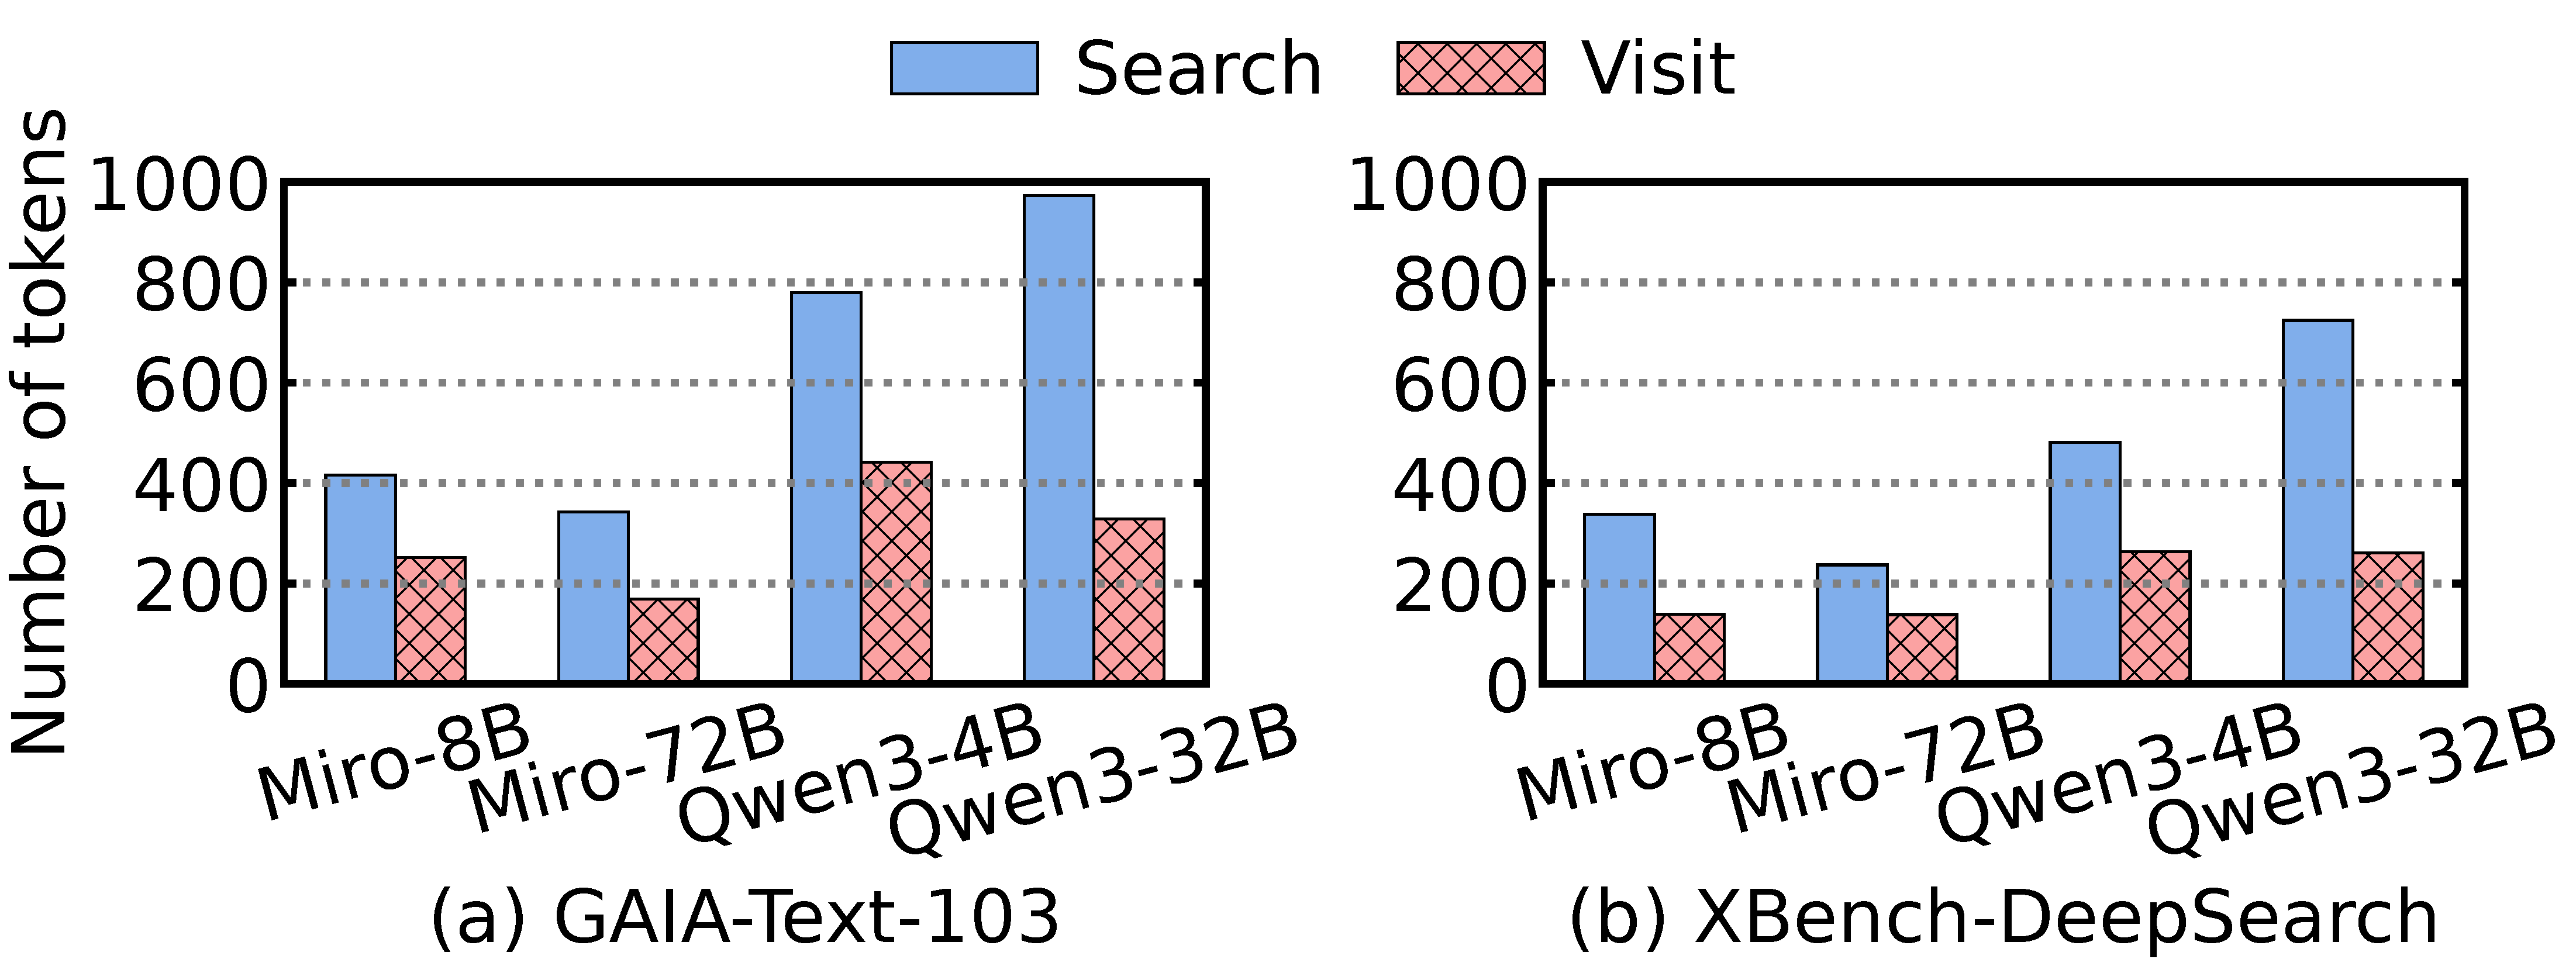
\includegraphics[width=\linewidth]{figs/token_count.pdf}
    \caption{Average reasoning length for generating Search and Visit actions across models and benchmarks. Search requires significantly longer reasoning than Visit.}
    \label{fig:motivation_tokens}
\end{figure}

\paragraph{Observation 1: Search actions involve longer reasoning traces than Visit.} 
Figure~\ref{fig:motivation_tokens} shows the average reasoning length before emitting an action. Across all models, Search consistently requires $1.65$--$2.95$$\times$ more tokens than Visit, indicating that query formulation inherently demands more deliberation than webpage selection. Therefore, Search actions carry stronger reasoning requirements.


% \paragraph{Observation 2: Effective speculation requires different strategies for Search and Visit.} 
% We measure alignment of the generated action using lightweight speculative methods with an Oracle agent (large model with full reasoning). Two representative strategies are compared: a small language model (SLM) with explicit reasoning, and a large language model (LLM) that skips reasoning 

% As shown in Figure~\ref{fig:motivation_alignment}(a),
% for Search actions, the small reasoning model consistently produces queries more aligned with the Oracle than the large model without reasoning, quantified via embedding-based cosine similarity~\cite{reimers-2019-sentence-bert}. Therefore, explicit reasoning is critical for query quality, even with reduced model capacity.
% In contrast, Figure~\ref{fig:motivation_alignment}(b--c) demonstrates that, to generate Visit actions, the large model skipping reasoning aligns more closely with the Oracle in both URL selection and extraction instruction. This indicates that deliberative reasoning is less crucial for Visit, where fast, pattern-based selection with large model capacities suffices.

\paragraph{Observation 2: Effective speculation strategies differ across actions.}
We measure the alignment of speculative actions with an Oracle agent (large model with full reasoning) using two representative strategies: a small language model (SLM) with explicit reasoning and a large language model (LLM) that skips reasoning.
As shown in Figure~\ref{fig:motivation_alignment}(a), for Search actions, the SLM with reasoning consistently produces queries more aligned with the Oracle than the LLM without reasoning, measured via embedding-based cosine similarity~\cite{reimers-2019-sentence-bert}. This indicates that explicit reasoning is critical for query quality even under reduced model capacity. In contrast, Figure~\ref{fig:motivation_alignment}(b--c) shows that for Visit actions, the LLM without reasoning aligns more closely with the Oracle in both URL selection and extraction instruction, suggesting that deliberative reasoning is less essential for Visit, where pattern-based selection benefits more from model capacity.
\begin{figure}
    \centering
    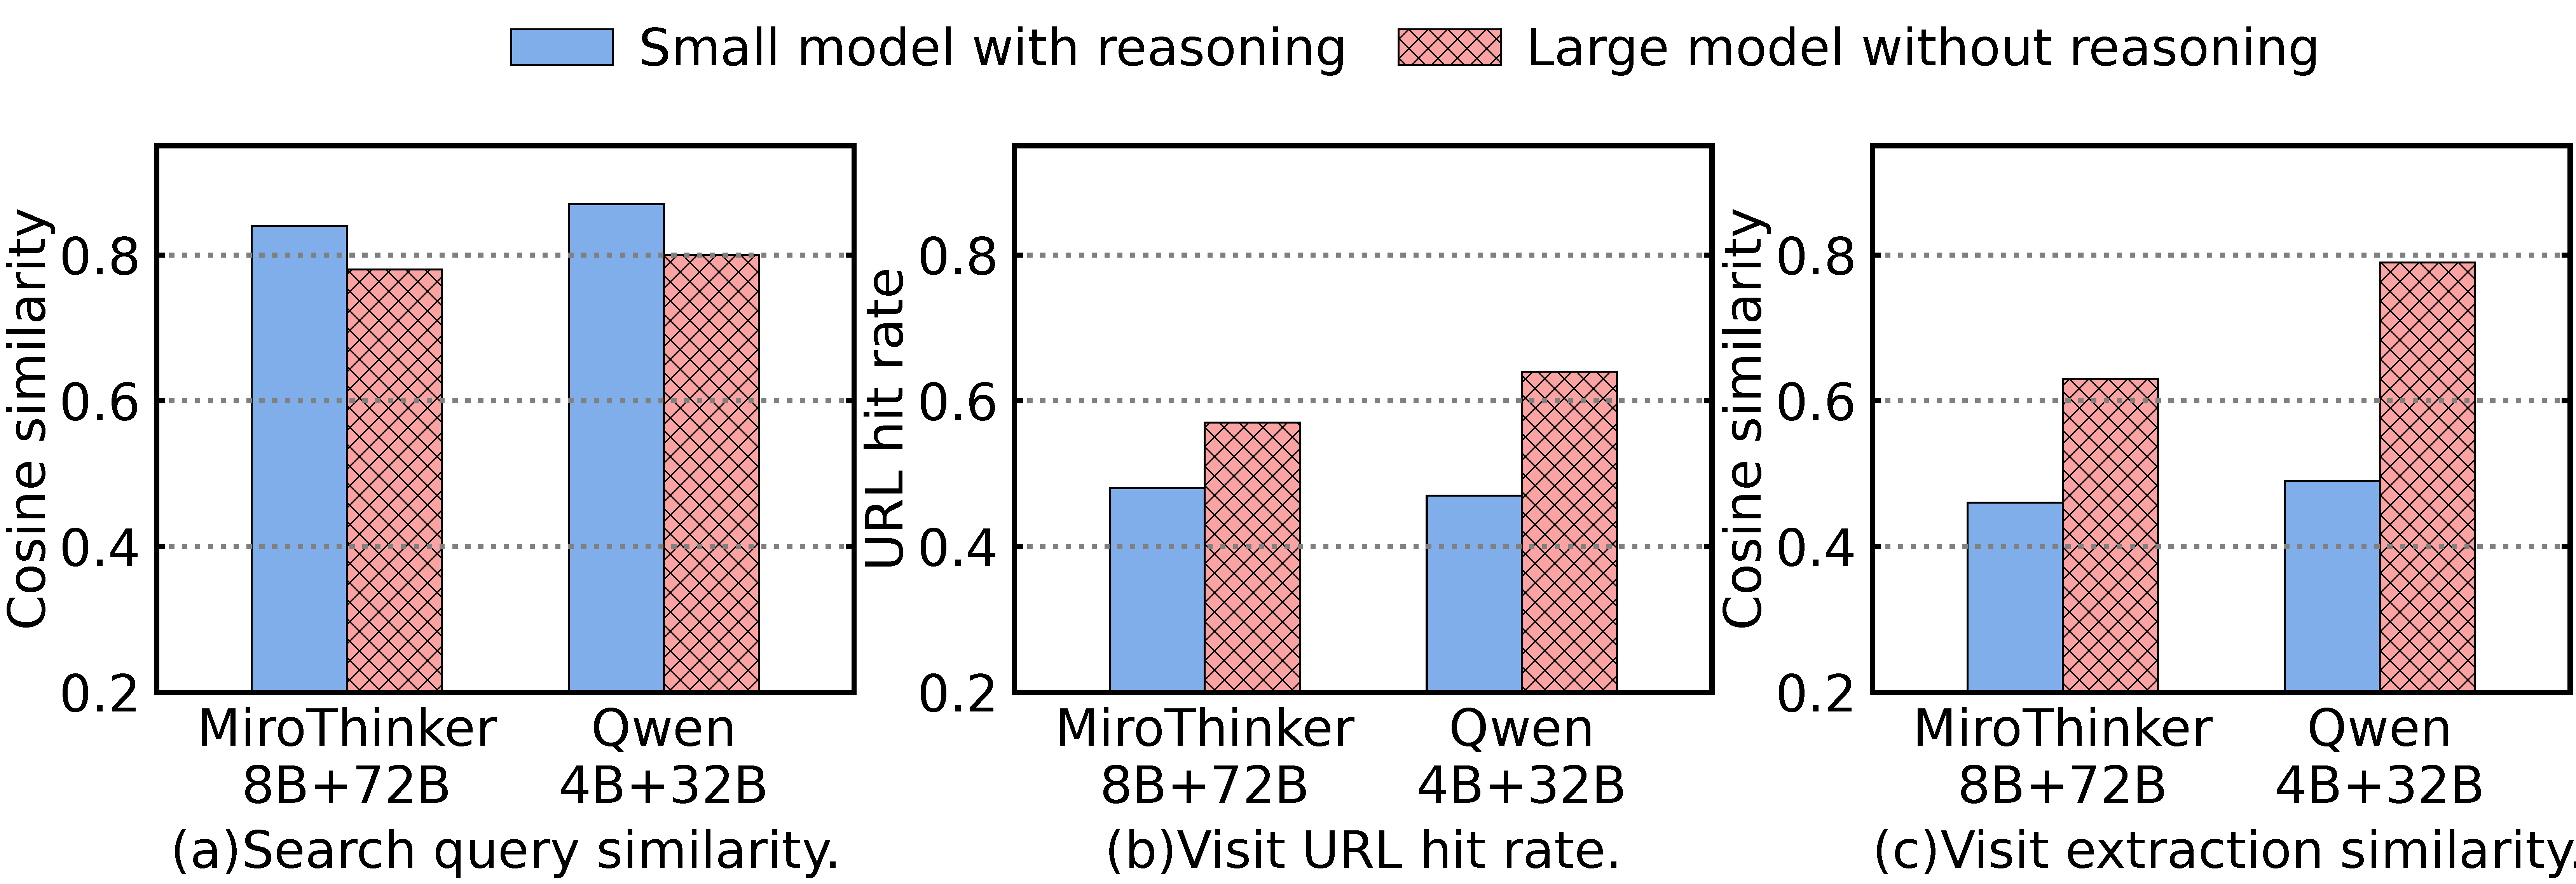
\includegraphics[width=\linewidth]{figs/motivation_similarity.pdf}
    \caption{Action alignment comparison of two speculative methods relative to the Oracle (large model with reasoning) when drafting Search and Visit. (a) The small reasoning model produces  queries more aligned with the Oracle than the large model without reasoning. (b--c) For Visit, the large model skipping reasoning achieves higher accuracy in both URL selection and extraction instruction.}
    \label{fig:motivation_alignment}
\end{figure}

\begin{table}[t]
    \centering
    \caption{End-to-end agent performance (pass@1 accuracy) on GAIA under action-level replacements.
We selectively replace the generation strategy for Search or Visit using lightweight methods.}
    \label{tab:action}
    {\small
    \begin{tabularx}{\columnwidth}{Xcc}
        \toprule
        Configuration & MiroThinker & Qwen3 \\
        \midrule
        LLM with Reasoning        & \textbf{63.11} & \textbf{29.13} \\
        \hdashline
        SLM with Reasoning for Search     & \textbf{63.11} & \textbf{29.13} \\
        LLM without Reasoning for Search  & 57.28 & 23.30 \\
        SLM without Reasoning for Search  & 55.34 &  22.33 \\
        \hdashline
        SLM with Reasoning for Visit      & 56.31 & 22.33 \\
        LLM without Reasoning for Visit   & \textbf{64.08} & \textbf{28.16} \\
        SLM without Reasoning for Visit  & 54.37 & 24.27 \\
        \bottomrule
    \end{tabularx}
    }
\end{table}


% To assess how different lightweight draft methods impact the end-to-end agent performance, we perform action-level interventions that selectively replace the generated action using a lightweight method, while keeping the remainder of the agent pipeline unchanged. We also consider a third option that combines both reduced model capacity and reasoning depth (SLM without reasoning).

% Table~\ref{tab:action} shows the results.
% Assigning small reasoning model to \textit{Search} preserves end-to-end accuracy, whereas 
% using a large model without reasoning degrades performance.
% Conversely, generating \textit{Visit} with a large model skipping reasoning achieves the best results, while another option leads to significant accuracy drops.
% Interestingly, although Figure~\ref{fig:motivation_alignment} demonstrates that the speculation cannot perfectly align with the Oracle at the action level, the end-to-end 
% accuracy can still be well maintained when right inference pathways are chosen for different actions.

To assess end-to-end effects, we perform action-level interventions that selectively replace Search or Visit generation with lightweight methods while keeping the rest of the pipeline unchanged. We also include another variant of speculation combining reduced capacity and reduced reasoning (SLM without reasoning).
Table~\ref{tab:action} shows that assigning an SLM with reasoning to \textit{Search} preserves overall accuracy, whereas using an LLM without reasoning degrades performance. Conversely, generating \textit{Visit} with an LLM without reasoning yields the best results, while alternative choices lead to significant accuracy drops. Although speculative actions do not perfectly align with the Oracle (Figure~\ref{fig:motivation_alignment}), 
end-to-end accuracy remains high because of the tolerance of approximation in reasoning models, as long as appropriate inference pathways are chosen per action.


% end-to-end accuracy remains high when appropriate inference pathways are chosen per action.



% \paragraph{Key insight: Search as System~2, Visit as System~1.}
% Taken together, these observations reveal a clear dichotomy between action types.
% We interpret this through the lens of dual-process theory.
% Search aligns with System~2 behavior: it requires deliberative reasoning to bridge the gap between an underspecified research objective and an effective query.
% In contrast, Visit aligns with System~1 behavior: given a set of candidates, selection and extraction rely primarily on fast, intuitive pattern recognition encoded in the model's parametric knowledge.
% This distinction provides a principled foundation for action-aware speculation.

\paragraph{Key insight: Search as System~2, Visit as System~1.}
These results reveal a clear action-level dichotomy. Viewed through dual-process theory, Search exhibits System~2 behavior, requiring deliberative reasoning to translate underspecified research goals into effective queries. Visit aligns with System~1 behavior, where selection and extraction primarily rely on fast, pattern-based recognition encoded in model parameters. This distinction provides a principled foundation for action-aware speculation.


% \subsection{Verification Beyond Action Matching}
% Speculation alone is insufficient for reliable speedups; verification is critical to prevent error propagation. Existing approaches typically verify speculative actions via exact or approximate action matching against the base model output. However, this strategy has two limitations.

% First, defining action equivalence is non-trivial. Exact matching is overly restrictive: 
% semantically equivalent Search queries may differ at the token level, leading to unnecessary rejection. 
% Approximate matching often requires additional modules (e.g., embedding models) and threshold tuning, complicating systems design.

% Second, verification usually requires the base model to complete its reasoning trace, placing it on the critical path and limiting latency reduction. More aggressive speculate-verify designs~\cite{guan2025dynamic} allow speculation to continue multiple steps for parallel verification, but failure in the middle requires rolling back all speculative steps, wasting computation.
% Therefore, achieving better accuracy-efficiency trade-offs demands verification strategies that go beyond simple action matching.

\subsection{Verification Beyond Action Matching}
Speculation alone is insufficient for reliable speedups; verification is essential to prevent error propagation. Most existing methods verify speculative actions via exact or approximate matching with the base model output, but this has two limitations.
First, action equivalence is hard to define. Exact matching is overly restrictive, as semantically equivalent Search queries may differ token-wise, causing unnecessary rejection, while approximate matching often requires additional modules (e.g., embedding models) and threshold tuning.
Second, verification typically places the base model's full reasoning trace on the critical path, limiting latency gains. More aggressive designs~\cite{guan2025dynamic} allow multi-step speculation with parallel verification, but failures in the middle require rolling back all following speculative steps, wasting computation. Achieving better accuracy-efficiency trade-offs therefore requires verification strategies beyond simple action matching.
 





\iffalse

\subsection{Speculation Under Action Heterogeneity}

To reduce the cost of agents, existing systems typically adopt two forms of speculation: reducing reasoning or reducing model capacity by using smaller models.
These strategies are commonly applied uniformly across all actions.
In this section, we examine how they affect different action types, and show that their effectiveness is highly action-dependent.
We present a set of empirical observations that motivate our key hypothesis that different actions exhibit different sensitivities to reasoning and model capacity.

\begin{figure}
    \centering
    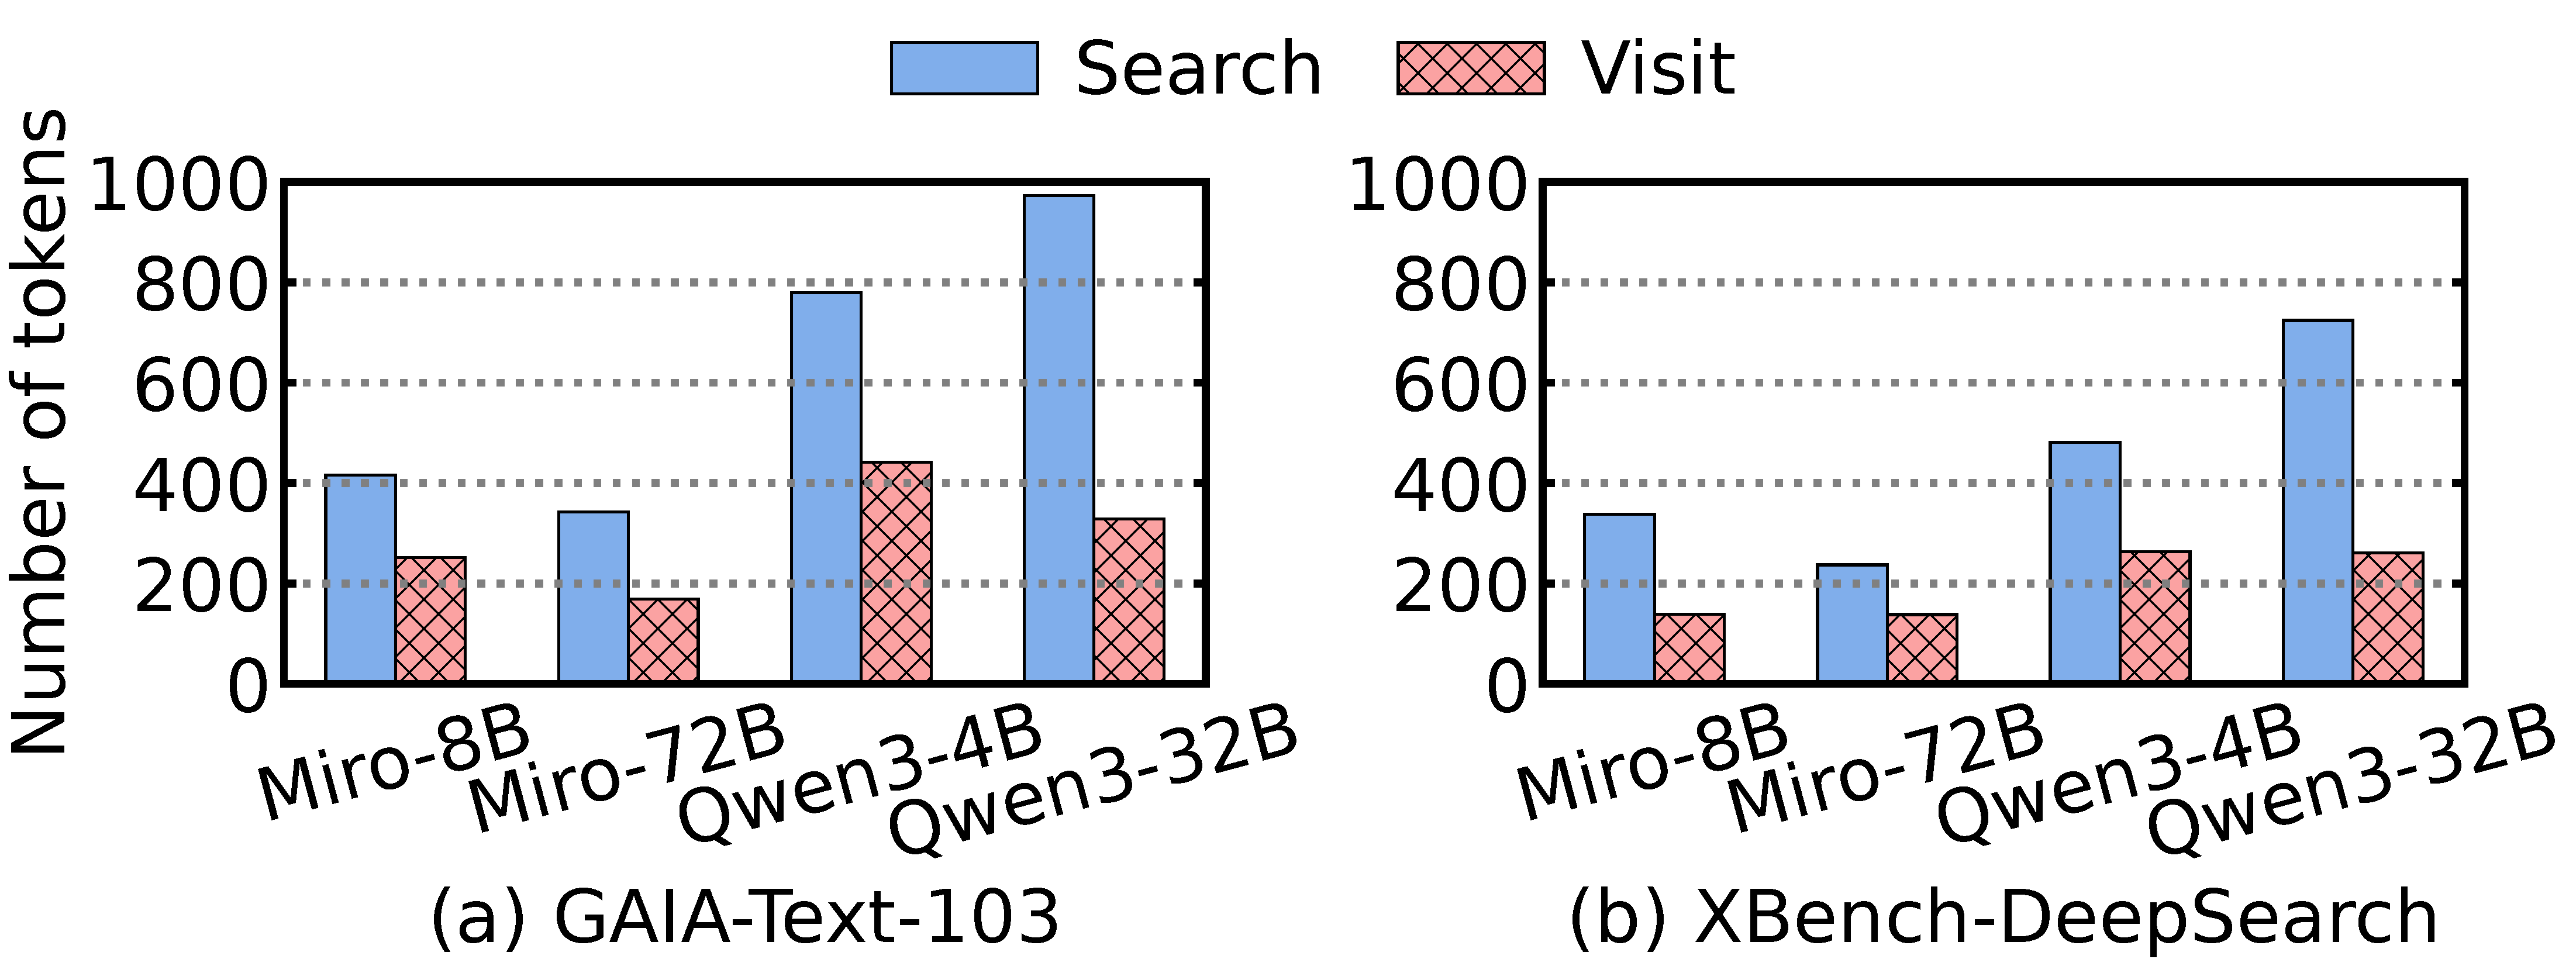
\includegraphics[width=\linewidth]{figs/token_count.pdf}
    \caption{Comparison of reasoning length for generating \textit{Search} and 
    \textit{Visit} actions on different benchmarks. \textit{Search} requires longer reasoning length than \textit{Visit}.}
    \label{fig:motivation_tokens}
\end{figure}

\paragraph{Observation 1: Search is preceded by longer reasoning traces than Visit.}
We observe a consistent gap in the amount of pre-action generation across action types.
As illustrated in Figure~\ref{fig:motivation_tokens}, the number of tokens produced before emitting a \textit{Search} action is consistently larger than that before a \textit{Visit} action across models and benchmarks.
This result indicates that models tend to spend more tokens before committing to Search than Visit within the same deep research workflow.

% \bt{Search naturally needs more reasoning tokens than visit.}

\begin{figure}
    \centering
    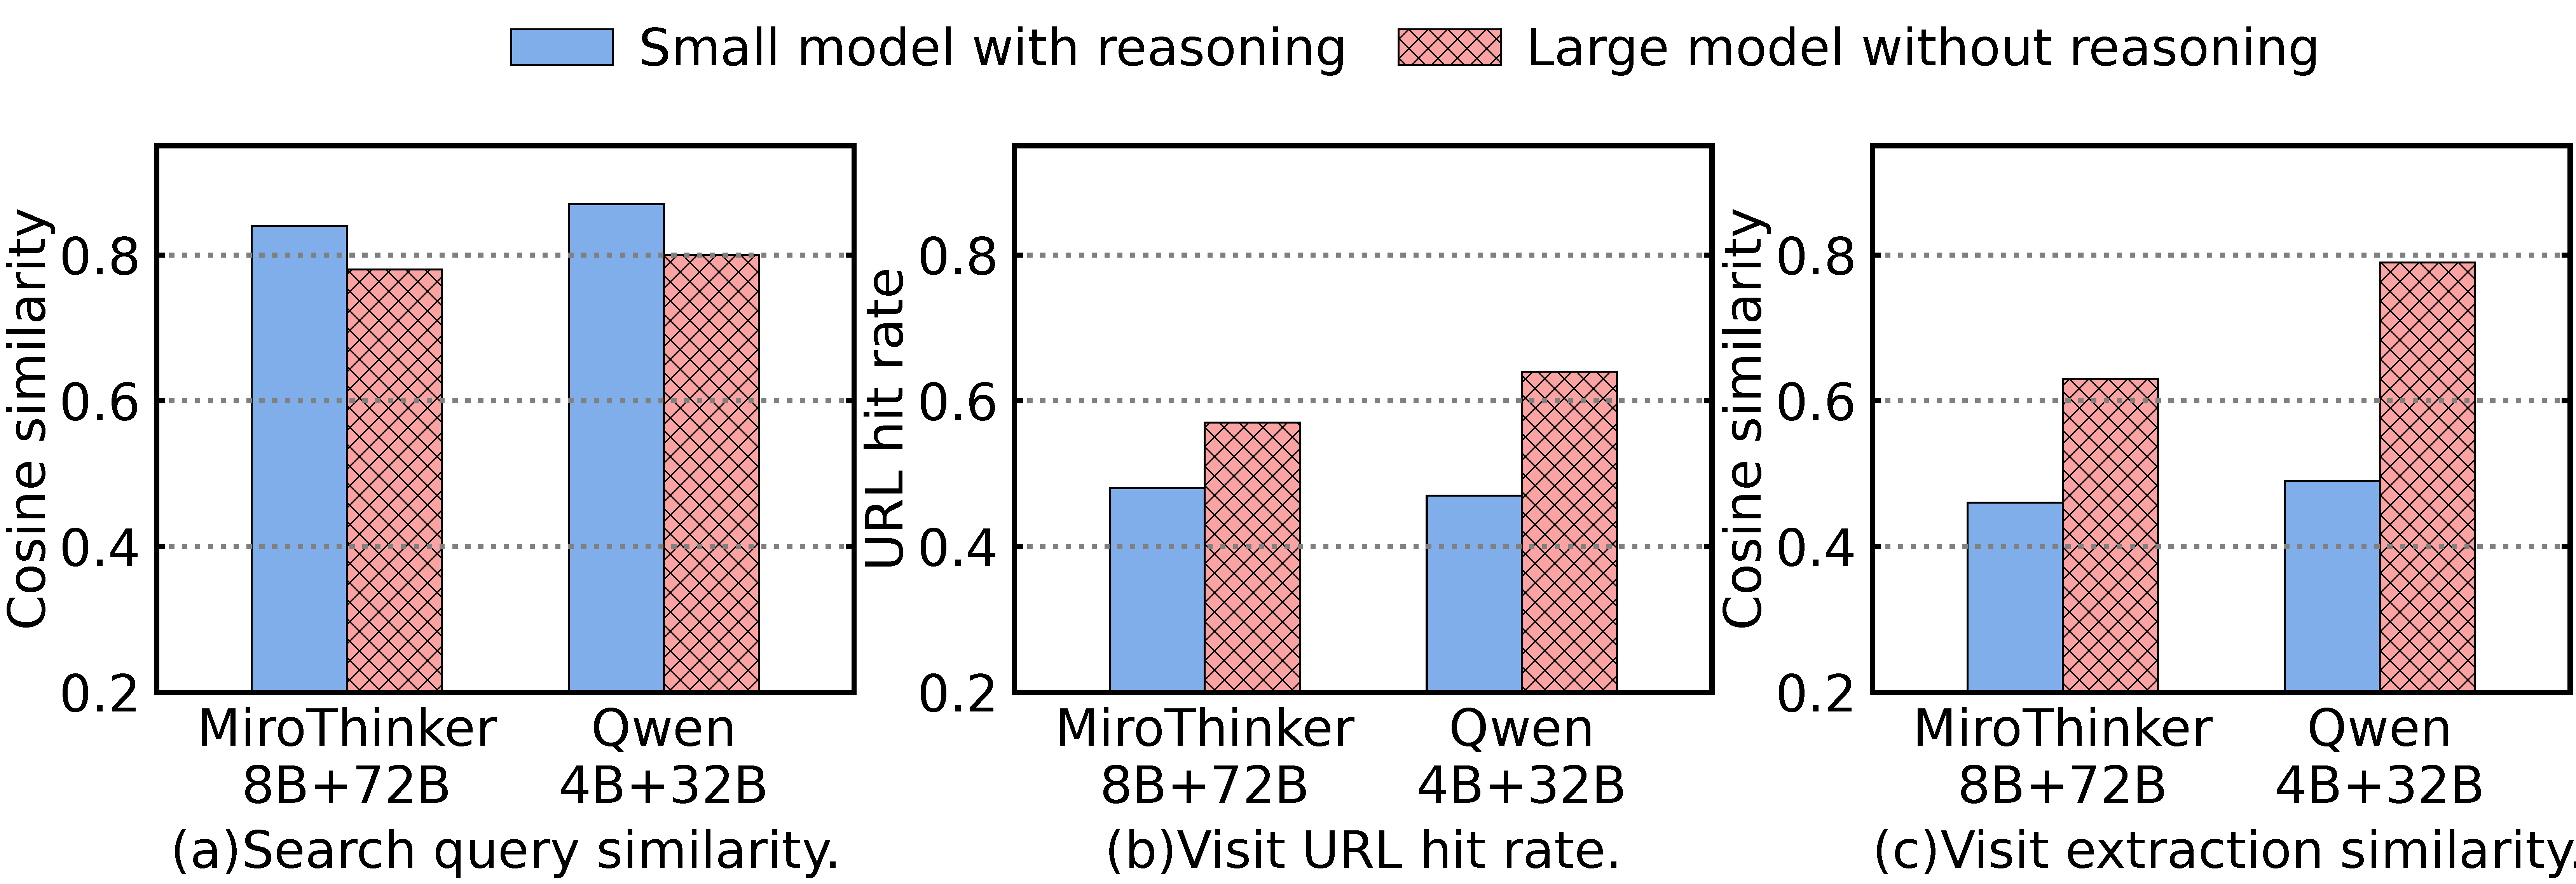
\includegraphics[width=\linewidth]{figs/motivation_similarity.pdf}
    \caption{Action alignment comparison of two lightweight methods relative to the Oracle (large model with reasoning). (a)(c) For Search queries and Visit extraction infos, we use the embedding-based cosine similarity between the generated query and the Oracle’s query. (b) For Visit URLs, alignment is evaluated using the direct hit rate against the Oracle’s selection.}
    \label{fig:motivation_alignment}
\end{figure}

\paragraph{Observation 2: Asymmetric Alignment Requirements for Search and Visit.}
We find that the requirements for maintaining behavioral alignment with the Oracle (Large Model with full reasoning) are fundamentally different for Search and Visit actions.

Specifically, for Search actions, a small model with reasoning aligns more closely with the Oracle than a Large Model without reasoning. We measure alignment by calculating the cosine similarity of the embeddings of the generated search queries with a a pre-trained embedding model. As shown in Figure~\ref{fig:motivation_alignment}(a), across the two model series, small model with reasoning can generate quereis that are more consistent with the reference compared with large model without reasoning.

In contrast, for Visit actions, a Large Model skipping reasoning aligns more closely with the Oracle than small model with reasoning. We evaluate alignment through two specialized metrics for the the target URL selection and the information extraction instruction in the visit arguments. For URL selection, we measure the direct hit rate against the Oracle’s chosen link. For extraction instructions, we compute the cosine similarity between the embeddings of the generated text and the Oracle’s reference, mirroring our evaluation of Search queries. As illustrated in Figure~\ref{fig:motivation_alignment}(b)(c), the alignment peaks when the large model is used.

\begin{table}[h]
    \centering
    \caption{End-to-end accuracy on gaia-text-103 under action-level replacements.
We selectively modify the generation strategy for \textsc{Search} or \textsc{Visit} while keeping the rest unchanged.}
    \label{tab:placeholder_label}
    \begin{tabular}{ccc}
        \toprule
        Configuration & MiroThinker& Qwen3 \\
        \midrule
        Large Model                 & \textbf{63.11} & \textbf{29.13} \\
        Small Model For Search      & \textbf{63.11} & \textbf{29.13} \\
        Small Model For Visit       & 56.31 & 22.33 \\
        Skip Reasoning For Search   & 57.28 & 22.33 \\
        Skip Reasoning For VISIT    & \textbf{64.08} & \textbf{28.16} \\
        Small + Skip  For Search    &  &  \\
        Small + Skip  For VISIT    & 54.37 &  \\
        \bottomrule
    \end{tabular}
\end{table}

\paragraph{Observation 3:}
We take action-level interventions that replace only the action generation module while keeping the rest of the agent pipeline unchanged.
As shown in Table~\ref{tab:placeholder_label}, assigning reasoning to \textsc{Search} preserves end-to-end accuracy, while skipping reasoning for \textsc{Visit} does not hurt the performance. These results indicate that once actions are generated under appropriate inference pathways, maintaining accuracy does not hinge on enforcing strict per-step alignment.

\paragraph{Key Insight: Search as System~2, Visit as System~1.}
Building upon these observations, we hypothesize that Search and Visit place fundamentally different demands on a model's inference process. We frame this distinction through the lens of dual-process theory: Search aligns with System 2 behavior, where deliberative reasoning is essential to bridge the "reasoning gap" between an underspecified research goal and an effective query. Conversely, Visit corresponds to System 1 behavior; once candidate results are presented, the selection and extraction process is more direct, relying on the model’s internal parametric knowledge rather than explicit logical deduction.

\subsection{Verification Beyond Exact Action Matching}

\noindent \textbf{Principle~2: Lightweight semantic verification.}
Rather than enforcing strict action-level equivalence at every step, high end-to-end accuracy can be achieved through lightweight semantic verification.
Specifically, each generated action can be evaluated by a full-capacity model using a coarse-grained consistency check with respect to the overall reasoning trajectory, without requiring exact matching to a reference output.
As long as the action is deemed semantically consistent, it can be accepted, reserving full regeneration for cases where substantial deviation is detected.

\fi


% \noindent \textbf{Principle~1: Heterogeneous Action Generation.}
% This System~1/System~2 distinction suggests a simple design principle: inference should be heterogeneous across actions.
% Actions that align with System~2 behavior should be generated with explicit reasoning to support deliberative decision making, while System~1 actions can be generated directly by a strong model without additional reasoning.
% Concretely, this motivates assigning reasoning, even with a smaller model, to \textsc{Search}, and executing \textsc{Visit} with a full-size model while skipping explicit reasoning.
\section{Theoretical Analysis}
\label{sec:theory}

% This section provides a theoretical perspective that explains the empirical findings in Section~\ref{sec:motivation}.
% We analyze why different actions in deep research agents exhibit fundamentally different sensitivities to explicit reasoning, and why this leads to distinct optimal speculation pathways.

% Our central claim is that Search and Visit actions differ in their intrinsic decision uncertainty.
% Explicit reasoning reduces uncertainty by introducing intermediate structure, but its benefit depends on the property of the action type.
% We formalize this intuition using an entropy-based analysis of action policies and show that Search actions admit significantly larger uncertainty reduction from reasoning than Visit actions.
% This provides a theoretical explanation for the System~2 vs.\ System~1 dichotomy observed empirically.

This section provides a theoretical explanation for the empirical observations in Section~\ref{sec:motivation}.
We analyze why different actions exhibit distinct sensitivities to explicit reasoning, leading to different optimal speculation strategies.

Our central claim is that Search and Visit actions differ in intrinsic decision uncertainty.
% While explicit reasoning reduces uncertainty by introducing intermediate structure, its effectiveness depends on the action type.
We formalize this intuition via an entropy-based analysis of action policies and show that Search actions benefit significantly more from reasoning-induced uncertainty reduction than Visit actions, explaining the empirically observed System~2 versus System~1 dichotomy.


\subsection{Preliminaries: Action Policies and Entropy}

At each step, an agent observes a state $s$ from the accumulated context and then samples an action $a$ 
from a policy $\pi(\cdot \mid s)$.
We denote the action spaces corresponding to Search and Visit by $\mathcal{A}_{\textsc{search}}$ and $\mathcal{A}_{\textsc{visit}}$, respectively.



A natural measure of decision uncertainty is the conditional entropy of the action policy:
\begin{equation}
H(\pi(\cdot \mid s)) \;=\; -\sum_{a \in \mathcal{A}} \pi(a \mid s)\log \pi(a \mid s).
\label{eq:policy_entropy}
\end{equation}
Lower entropy indicates a more confident and concentrated decision, whereas higher entropy reflects ambiguity among many plausible actions.

In deep research agents, however, actions are expressed as open-ended language strings (e.g., search queries or extraction instructions), rendering exact computation of~\eqref{eq:policy_entropy} intractable.
We therefore adopt a token-level proxy based on the negative log-likelihood of the realized action.
Specifically, for an action represented as a token sequence $a=(t_1,\ldots,t_n)$, we define the mean token-level entropy proxy:
\begin{equation}
\bar{H}(a \mid s) \;=\; \frac{1}{n}\sum_{i=1}^n \left(-\log p(t_i \mid s, t_{<i})\right),
\label{eq:token_entropy_proxy}
\end{equation}
where smaller $\bar{H}(a \mid s)$ (i.e., higher average token log probability) indicates lower decision uncertainty.


\subsection{Intrinsic Entropy Gap Between Search and Visit}

We first examine the baseline uncertainty of different actions when generated \emph{without} explicit reasoning.
Intuitively, Search actions map a broad and ambiguous intent to a concrete query, for which many formulations may be reasonable.
In contrast, Visit operates on retrieved candidates and localized content, significantly constraining the decision space.

\begin{figure}
    \centering
    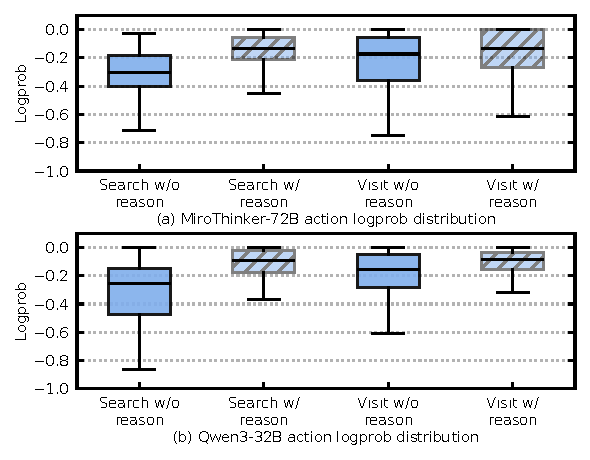
\includegraphics[width=\linewidth]{figs/logprob.pdf}
    \caption{Action log probability distributions with and without reasoning. 
    % We report the distribution of per-action mean token log probabilities for Search and Visit under two inference modes.
    A higher log probability indicates lower uncertainty.
    Without reasoning (dark blue color), Search actions exhibit lower log probabilities than Visit actions, indicating higher baseline decision uncertainty. 
    When reasoning is incorporated (light blue color with hatching), both action types see increased log probabilities, but the increase is significantly larger for Search actions, reflecting a greater reduction in uncertainty due to reasoning.}
    \label{fig:entropy_boxplot}
\end{figure}

This intuition is reflected in the following inequality:
\begin{equation}
    \mathbb{E}[\bar H(a\mid s)\mid a\in\mathcal{A}_{\textsc{search}}]
\;>\;
\mathbb{E}[\bar H(a\mid s)\mid a\in\mathcal{A}_{\textsc{visit}}].
\end{equation}
That is, under identical inference settings, Search actions exhibit higher average uncertainty than Visit actions.
Figure~\ref{fig:entropy_boxplot} visualizes this gap.
Each boxplot shows the distribution of mean token log probabilities for Search and Visit actions. 
When generated without reasoning, 
Search consistently exhibits lower log probabilities (higher $\bar{H}$) than Visit, suggesting less confident action distribution.


\subsection{Why Reasoning Helps: Entropy Reduction via Intermediate Structure}

We model explicit reasoning as the introduction of an intermediate latent variable $z$, corresponding to a reasoning trace that refines the decision context before the final action is generated.
This transforms the direct mapping $\pi(a \mid s)$ into a two-stage generation process:
\begin{equation}
\pi(a \mid s) \;=\; \sum_{z} \pi(z \mid s)\,\pi(a \mid s, z),
\label{eq:latent_factorization}
\end{equation}
where the final action is conditioned not only on the original state $s$, but also on the intermediate reasoning state $z$.
By a standard information-theoretic property~\cite{cover1999elements}, conditioning cannot increase entropy.
Formally,
\begin{equation}
\mathbb{E}_{z\sim \pi(\cdot\mid s)}\!\left[ H(\pi(\cdot \mid s, z)) \right] \;\le\; H(\pi(\cdot \mid s)).
\label{eq:entropy_reduction}
\end{equation}
Thus, access to a reasoning trace reduces action uncertainty and increases the likelihood of the realized action.


As shown in Figure~\ref{fig:entropy_boxplot}, incorporating reasoning consistently increases log probabilities, corresponding to a reduction in action-level uncertainty.
This reduction is most pronounced when the target decision relies on non-local associations that are not directly specified in the immediate input~\cite{prystawski2023think}.
Therefore, for Search, reasoning decomposes a global, underspecified mapping into a sequence of more localized sub-decisions, yielding a large reduction in uncertainty.
In contrast, Visit actions already exhibit low baseline entropy due to strong grounding in retrieved content.
Therefore, conditioning on an reasoning trace yields only a marginal additional reduction in uncertainty.


Taken together, this analysis explains why Search aligns more closely with \emph{System~2} behavior, while Visit is closer to \emph{System~1} behavior in deep research agents.



% this analysis explains the asymmetric benefit of reasoning observed in Section~\ref{sec:motivation}.
% Search actions operate in a high-entropy regime, where explicit reasoning plays a critical role in reducing uncertainty and improving decision quality.
% Visit actions, by contrast, operate in a low-entropy regime, where direct inference with sufficient model capacity is more helpful.
% This distinction closely mirrors the System~2 vs.\ System~1 dichotomy from dual-process theory.





\iffalse

Initial draft:

This section analyzes the underlying factors that differentiate \textit{System~2} and \textit{System~1} actions in deep research agents.
Specifically, we study why some actions benefit substantially from additional reasoning to reduce decision uncertainty, whereas others can be reliably produced by directly operating on concrete inputs.
To this end, we conduct an entropy-based analysis that quantifies action-level uncertainty and connects it to different inference pathways.

\subsection{Preliminaries: Action Policy and Entropy}
At each step, an agent observes a state $s$ (previous context) and samples an action $a \sim \pi(\cdot \mid s)$.
We denote the corresponding action sets of \textsc{Search} and \textsc{Visit} by $\mathcal{A}_{\textsc{search}}$ and $\mathcal{A}_{\textsc{visit}}$, respectively.

A natural measure of decision uncertainty is the conditional entropy of the action policy:
\begin{equation}
H(\pi(\cdot \mid s)) \;=\; -\sum_{a \in \mathcal{A}} \pi(a \mid s)\log \pi(a \mid s).
\label{eq:policy_entropy}
\end{equation}
However, in deep research agents, actions are emitted as open-ended natural-language strings (e.g., queries and URLs), making $H(\pi(\cdot \mid s))$ intractable to compute exactly.
We therefore use the per-token negative log-likelihood of the realized action as a tractable uncertainty proxy.
Concretely, for an action rendered as tokens $a = (t_1,\ldots,t_n)$, we compute
\begin{equation}
\bar{H}(a \mid s) \;=\; \frac{1}{n}\sum_{i=1}^n \left(-\log p(t_i \mid s, t_{<i})\right),
\label{eq:token_entropy_proxy}
\end{equation}
where a smaller $\bar{H}(a\mid s)$ (equivalently, a higher mean token log probability) indicates lower decision uncertainty.


\subsection{Entropy Gap Between \textsc{Search} and \textsc{Visit}}

We then compare action uncertainty under inference with and without explicit reasoning.
Intuitively, \textsc{Search} transforms a broad and ambiguous intent into a concise query, offering many plausible outputs. In contrast, \textsc{Visit} operates on returned content and often involves simpler decisions like selecting or extracting information, which inherently reduces ambiguity.


Our empirical findings confirm this intuition: in the absence of explicit reasoning,
\begin{equation}
    \mathbb{E}[\bar H(a\mid s)\mid a\in\mathcal{A}_{\textsc{search}}]
\;>\;
\mathbb{E}[\bar H(a\mid s)\mid a\in\mathcal{A}_{\textsc{visit}}].
\end{equation}
demonstrating an intrinsic entropy gap between \textsc{Search} and \textsc{Visit} actions.

\begin{figure}
    \centering
    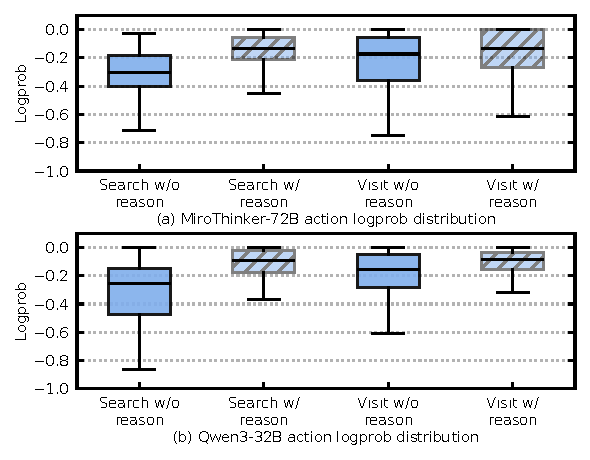
\includegraphics[width=\linewidth]{figs/logprob.pdf}
    \caption{Action log probability distributions with and without reasoning. We report the distribution of per action mean token log probabilities for \textsc{Search} and \textsc{Visit} under two inference modes. Results are shown for (a) MiroThinker-72B and (b) Qwen3-32B. \textsc{Visit} actions exhibit higher log probabilities even when generated without reasoning, suggesting lower baseline decision uncertainty.
    Consequently, the increase in action log probability brought by reasoning is substantially larger for \textsc{Search} than for \textsc{Visit}.}
    \label{fig:entropy_boxplot}
\end{figure}

Figure~\ref{fig:entropy_boxplot} visualizes this baseline difference.
Each boxplot shows the distribution of mean token log probabilities for \textsc{Search} and \textsc{Visit} actions when generated without reasoning.
Compared to \textsc{Visit}, \textsc{Search} consistently exhibits lower log probabilities (higher $\bar{H}$), suggesting larger decision uncertainty.

\subsection{Why Reasoning Helps: Entropy Reduction via Intermediate Structure}

We model explicit reasoning as introducing an intermediate latent variable $z$ (a reasoning trace) that refines the decision context before committing to the final action.
This transforms the direct mapping $\pi(a \mid s)$ into a two-stage generation process:
\begin{equation}
\pi(a \mid s) \;=\; \sum_{z} \pi(z \mid s)\,\pi(a \mid s, z),
\label{eq:latent_factorization}
\end{equation}
which can be viewed as marginalizing over possible reasoning traces.
By the standard property that conditioning cannot increase entropy, we have
\begin{equation}
\mathbb{E}_{z\sim \pi(\cdot\mid s)}\!\left[ H(\pi(\cdot \mid s, z)) \right] \;\le\; H(\pi(\cdot \mid s)),
\label{eq:entropy_reduction}
\end{equation}
suggesting that access to the latent trace $z$ reduces uncertainty and increases the likelihood of the final action.


As shown in Figure~\ref{fig:entropy_boxplot}, incorporating reasoning consistently increases action log probabilities, corresponding to a reduction in action-level uncertainty.
This reduction is most pronounced when the target decision relies on non-local associations that are not directly specified in the immediate input~\cite{prystawski2023think}.
In our setting, \textsc{Search} requires translating an abstract research goal into a concrete query, where many alternatives are plausible and the direct distribution is diffuse.
Reasoning introduces intermediate structure that decomposes this mapping into more localized sub-decisions, concentrating probability mass and yielding a larger reduction in uncertainty.

By contrast, \textsc{Visit} actions are more directly grounded in retrieved candidates and content, leading to a sharper action distribution even under non-reasoning inference.
As a result, additional reasoning yields a smaller marginal reduction in uncertainty.
Overall, these findings explain why \textsc{Search} aligns more closely with \emph{System~2} behavior, while \textsc{Visit} is closer to \emph{System~1} behavior in deep research agents.

\fi


% Putting the above together, we interpret \textsc{Search} as a \textit{System~2}-like action: it starts from a higher-entropy decision space and thus benefits more from explicit reasoning that reduces uncertainty before action emission.
% In contrast, \textsc{Visit} is \textit{System~1} action: its action entropy is naturally low, so additional reasoning yields limited marginal gain; performance instead depends on the model's parametric capacity to rapidly recognize and extract useful information from concrete inputs.


\section{\method{} Design}

\subsection{Overview}

\begin{figure}
    % [ht]
    \centering
    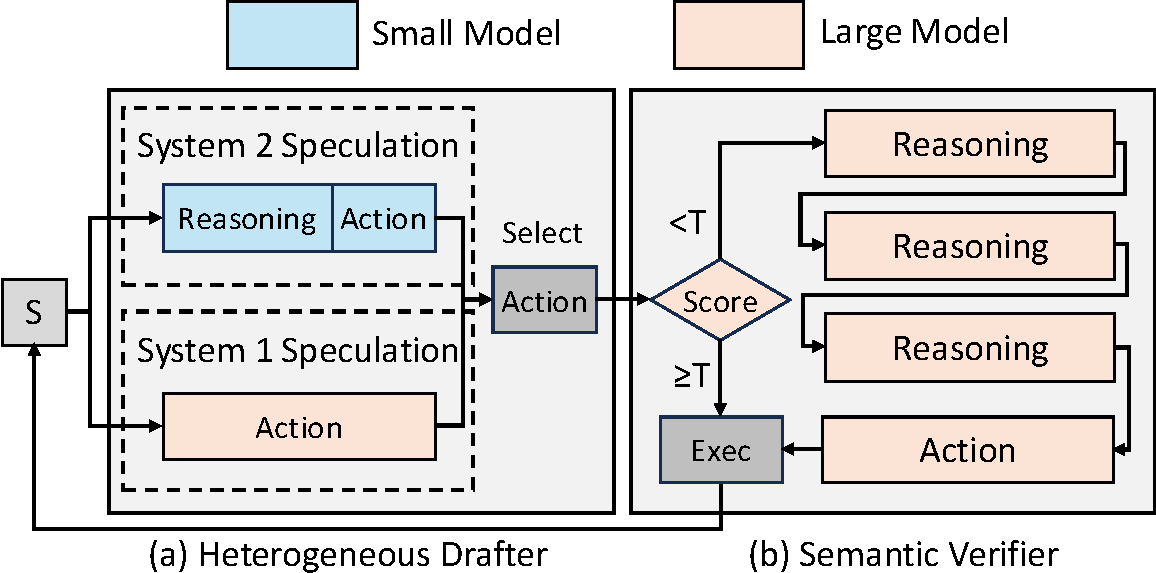
\includegraphics[width=\linewidth]{figs/overview.pdf}
    \caption{Overview of \method{}. 
    %  as an action-level speculative framework with heterogeneous drafting and semantic verification.
     }
    \label{fig:overview}
\end{figure}

We propose \method{}, a dual-process speculative framework for deep research agents.
The core design principle of \method{} is to allocate inference resources \emph{heterogeneously} across actions for high speculation accuracy, while preserving end-to-end agent performance through lightweight, step-wise semantic verification.

As illustrated in Figure~\ref{fig:overview}, \method{} follows a draft--verify workflow.
At each decision step, \method{} generates two candidate actions in parallel:
(i) a \textit{System~2} draft produced by a small model with explicit reasoning, and
(ii) a \textit{System~1} draft via a large model skipping reasoning.
The framework then selects a provisional draft based on the action type and the reasoning footprint from the small-model output.
Finally, the selected draft is evaluated by a semantic verifier using a full-capacity base model.
Drafts judged to be semantically consistent with the current reasoning trajectory are accepted and executed directly; otherwise, \method{} falls back to full-capacity reasoning to regenerate the action.

% Motivated by the observations and analysis, we propose \method{}, a dual-process speculative framework for deep research agents.
% \method{} is designed to allocate inference resources heterogeneously across actions while maintaining end-to-end accuracy through lightweight verification.

% As illustrated in Figure~\ref{fig:overview}, \method{} follows a draft--verify workflow.
% At each step, \method{} drafts two candidate actions in parallel: a \textit{System~2} draft from the small model with reasoning, and a \textit{System~1} draft from the large model without reasoning; it then selects between them using the action type and the draft’s reasoning footprint.
% The drafted action is then evaluated by a semantic verifier implemented with a full-capacity model.
% Actions that are judged to be consistent with the current reasoning trajectory are accepted and executed directly, whereas low-quality drafts trigger fallback to full-capacity reasoning.

\subsection{Heterogeneous Draft}
\label{subsec:hetero_draft}

% \method{} implements heterogeneous drafting by generating two candidate actions at each step and selecting the one that best matches the inference demand of the current decision.
% Given the current state $s_t$, we produce:
% (i) a \textit{System~2} draft $(z_s, a_s)$ using the small model with explicit reasoning, and
% (ii) a \textit{System~1} draft $a_l$ using the large model without explicit reasoning.
% The key question is how to select the final drafted action while preserving useful reasoning context.

\method{} implements heterogeneous drafting by producing two candidate actions at each step and adaptively selecting the one that best matches the inference demand of the current decision.
Formally, given the current state $s_t$, we generate a System~2 draft $(z_s, a_s)$ using SLM and
a System~1 draft $a_l$ using LLM.
The key question is how to select the final drafted action while retaining reasoning information that is valuable for long-horizon planning.


% We use the action type produced by the small-model draft as the primary routing signal.
% If the small model proposes a \textsc{Search} action, we keep $a_s$ as the draft action, since \textsc{Search} benefits from explicit reasoning and the small model is sufficient when paired with reasoning.
% If the small model proposes a \textsc{Visit} action, we typically replace it with the large-model no-reasoning draft $a_l$, since \textsc{Visit} relies more on the large model’s parametric capacity for direct decisions on concrete inputs.
\paragraph{Action-aware selection.}
We use the action type predicted by the small-model draft as the primary routing signal.
If the small model generates a Search action, we retain $a_s$ as the draft action, as Search typically benefits from explicit reasoning and can be reliably handled by a smaller model when paired with a reasoning trace.
If the small model proposes a Visit action, we instead select the large-model draft $a_l$ in most cases, since Visit actions rely more heavily on the large model's parametric capacity to make direct decisions on concrete inputs.

\paragraph{Preserving long-horizon reasoning.}
An important exception arises when the small-model draft produces a long reasoning trace before emitting its action.
Empirically, such extended reasoning often contains global analysis or intermediate summaries that remain useful beyond the current step, regardless of whether the final action is Search or Visit.
To preserve this information, when the length of the small-model reasoning exceeds a threshold $\tau_{\text{think}}$, we choose the full draft $(z_s, a_s)$ even if the action type is Visit.
This mechanism ensures that high-level reasoning is not discarded when it may benefit subsequent decisions.


\subsection{Semantic Verification}
\label{subsec:semantic_verification}


To maintain end-to-end accuracy, \method{} performs lightweight semantic verification at every step.
Instead of enforcing action-level matching, the verifier assesses whether the drafted reasoning and action are likely to make meaningful progress.
This design is motivated by the observation that intermediate agent decisions are often tolerant to approximation as illustrated in table~\ref{tab:action}.
Moreover, this approach avoids the reasoning delays from the base models to generate actions, enabling faster verification.   

Given the current state $s_t$ and a draft consisting of an optional reasoning trace $z_t$ and a candidate action $a_t$, we query the large model as a critic and ask it to answer \texttt{Yes} or \texttt{No}.
The prompt instructs the critic to jointly assess (i) whether the reasoning is coherent (if present) and (ii) whether the proposed action is useful for making progress.
The exact prompt template is provided in Appendix~\ref{app:verifier_prompt}.

Although the critic produces a discrete verdict, a \emph{continuous} signal is necessary to trade off speed and reliability.
We therefore convert the critic's output distribution into a real-valued confidence score.

Let $p_{\mathrm{acc}}(s_t,z_t,a_t)$ and $p_{\mathrm{rej}}(s_t,z_t,a_t)$ denote the critic's probabilities of answering \texttt{Yes} and \texttt{No}, respectively.
We define the verification score as the log-probability margin:
\begin{equation}
\mathrm{score}(s_t, z_t, a_t)
=
\log p_{\mathrm{acc}}(s_t, z_t, a_t)
-
\log p_{\mathrm{rej}}(s_t, z_t, a_t),
\label{eq:verifier_score}
\end{equation}
which corresponds to the log-odds of acceptance and provides a stable, monotonic measure of verifier confidence.

We accept the draft if its score exceeds a threshold $\tau$:
\begin{equation}
\textsc{Accept}(z_t, a_t)
\quad \text{if} \quad
\mathrm{score}(s_t, z_t, a_t) \ge \tau,
\label{eq:accept_rule}
\end{equation}
and otherwise trigger fallback.
Fallback regenerates the step using the full-capacity model with explicit reasoning and continues execution with the regenerated action.
This verification-and-fallback procedure follows a standard speculative pattern: propose a fast approximate step, validate it with a stronger critic, and only pay the cost of full reasoning when the draft is unlikely to be reliable.

Since the score scale depends on the critic model, we select $\tau$ offline on a held-out development set.
We sweep candidate thresholds and choose a fixed $\tau$ that preserves end-to-end accuracy while maximizing the acceptance rate, and keep it fixed at runtime.
This allows \method{} to allocate expensive full-capacity reasoning only to the minority of uncertain steps, improving overall time-to-solution. Additional empirical evidence on the effectiveness of this verifier score is provided in Appendix~\ref{app:verifier_scores}.




\iffalse

Motivated by the observations and analysis, we propose \method{}, a dual-process speculative framework for deep research agents.
\method{} is designed to allocate inference resources heterogeneously across actions while maintaining end-to-end accuracy through lightweight verification.

As illustrated in Figure~\ref{fig:overview}, \method{} follows a draft--verify workflow.
At each step, \method{} drafts two candidate actions in parallel: a \textit{System~2} draft from the small model with reasoning, and a \textit{System~1} draft from the large model without reasoning; it then selects between them using the action type and the draft’s reasoning footprint.
The drafted action is then evaluated by a semantic verifier implemented with a full-capacity model.
Actions that are judged to be consistent with the current reasoning trajectory are accepted and executed directly, whereas low-quality drafts trigger fallback to full-capacity reasoning.

\subsection{Heterogeneous Draft}
\label{subsec:hetero_draft}

\method{} implements heterogeneous drafting by generating two candidate actions at each step and selecting the one that best matches the inference demand of the current decision.
Given the current state $s_t$, we produce:
(i) a \textit{System~2} draft $(z_s, a_s)$ using the small model with explicit reasoning, and
(ii) a \textit{System~1} draft $a_l$ using the large model without explicit reasoning.
The key question is how to select the final drafted action while preserving useful reasoning context.

\paragraph{Action-aware selection.}
We use the action type produced by the small-model draft as the primary routing signal.
If the small model proposes a \textsc{Search} action, we keep $a_s$ as the draft action, since \textsc{Search} benefits from explicit reasoning and the small model is sufficient when paired with reasoning.
If the small model proposes a \textsc{Visit} action, we typically replace it with the large-model no-reasoning draft $a_l$, since \textsc{Visit} relies more on the large model’s parametric capacity for direct decisions on concrete inputs.

\paragraph{Preserving long-horizon reasoning.}
A subtle but important case arises when the small-model draft generates a long reasoning trace before emitting its action.
In practice, such long reasoning often contains global analysis or intermediate summaries that are useful for subsequent steps, regardless of whether the final action is \textsc{Search} or \textsc{Visit}.
Therefore, when the small-model reasoning length exceeds a threshold $\tau_{\text{think}}$, we preserve its reasoning trace even if the action type is \textsc{Visit}.
Concretely, we keep $(z_s, a_s)$ as the drafted output in this case, so that the accumulated context retains the small model’s high-level reasoning.


\subsection{Semantic Verification}
\label{subsec:semantic_verification}

 \method{} performs lightweight semantic verification at every step to preserve end-to-end accuracy.
Instead of enforcing strict action-level equivalence, the verifier checks whether the drafted reasoning and action are semantically consistent with the current trajectory and are likely to provide useful progress.
This follows the observation that intermediate decisions are tolerant to approximation as long as their semantic contribution is preserved, and that a strong model can efficiently assess such intermediate steps and trigger correction only when necessary.

Given the current state $s_t$ and a draft output consisting of an optional reasoning trace $z_t$ and a candidate action $a_t$, we query the full-size model as a critic to output a single binary judgment (\texttt{Yes} or \texttt{No}).
The prompt asks the critic to jointly assess whether the reasoning is consistent and whether the action is useful for progress.
When the draft pathway skips explicit reasoning, we set $z_t=\emptyset$.
We provide the exact prompt template in Appendix~\ref{app:verifier_prompt}.

Although the output is binary, the critic assigns probabilities to both acceptance and rejection.
We therefore derive a continuous verification score from the model distribution.
Let $p_{\mathrm{v}}(\cdot \mid s_t, z_t, a_t)$ denote the next-token distribution under the verifier prompt.
To ensure robustness to minor formatting and tokenizer variability, we aggregate probability mass over semantically equivalent affirmative and negative responses.
We define the verification score as the log-probability margin:
\begin{equation}
\mathrm{score}(s_t, z_t, a_t)
=
\log p_{\mathrm{acc}}(s_t, z_t, a_t)
-
\log p_{\mathrm{rej}}(s_t, z_t, a_t),
\label{eq:verifier_score}
\end{equation}
where $p_{\mathrm{acc}}$ and $p_{\mathrm{rej}}$ are the aggregated probabilities of affirmative and negative responses, respectively.


\paragraph{Acceptance rule and fallback.}
We accept the drafted output when its score exceeds a threshold $\tau$:
\begin{equation}
\textsc{Accept}(z_t, a_t)
\quad \text{if} \quad
\mathrm{score}(s_t, z_t, a_t) \ge \tau,
\label{eq:accept_rule}
\end{equation}
and otherwise trigger fallback.
Fallback regenerates the step using the full-size model with explicit reasoning and continues execution with the regenerated action.
This verification-as-scoring mechanism matches the speculative reasoning pattern of proposing an approximate step using a lightweight pathway, assessing it with a stronger model, and correcting it only when needed.

\paragraph{Threshold profiling.}
The score scale depends on the verifier model and tokenizer, so $\tau$ is model-dependent.
We therefore profile $\tau$ offline for each model pair on a held-out development set.
Concretely, we sweep candidate thresholds and choose a fixed $\tau$ that preserves end-to-end accuracy while maximizing acceptance rate, and keep $\tau$ fixed at runtime.
This allows \method{} to concentrate expensive full-capacity reasoning on the minority of steps where the draft is unlikely to be reliable, improving end-to-end time-to-solution.

\fi
\begin{figure*}[h]
    \centering
    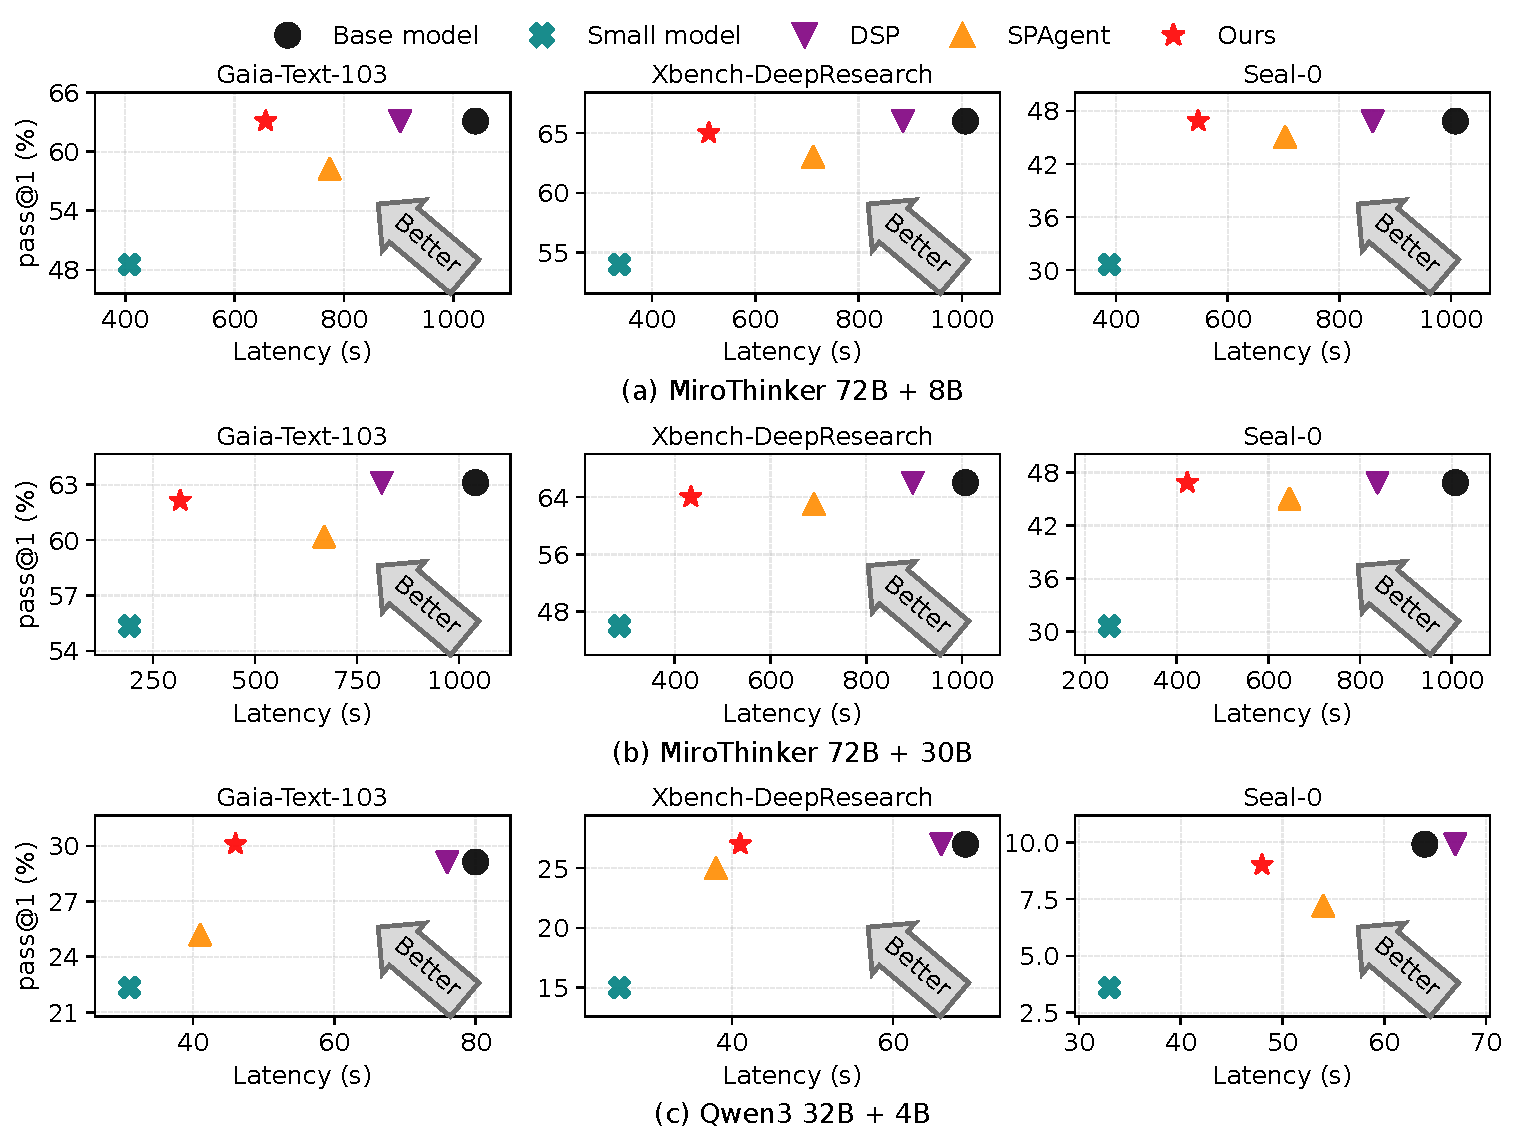
\includegraphics[width=0.9\linewidth]{figs/main_exp_results.pdf}
    \caption{Comparison of the accuracy (pass@1) and latency of different schemes across model combinations.
\method{} consistently reduces end-to-end latency by \textbf{1.33–3.28$\times$} (\(\sim\)2$\times$ on average) over the base model while maintaining comparable accuracy.
Compared with DSP and SPAgent, \method{} achieves a better accuracy–latency trade-off across all datasets and model pairs.}
    \label{fig:main_results}
\end{figure*}

\section{Experiments}

\subsection{Experimental Setup}

\paragraph{Models.}
We evaluate \method{} under three dual-model configurations: 
MiroThinker-v1.0-72B + MiroThinker-v1.0-8B, 
MiroThinker-v1.0-72B + MiroThinker-v1.0-30B-A3B, and 
Qwen3-32B + Qwen3-4B~\cite{team2025mirothinker,yang2025qwen3}. All models are deployed single-tenant with one \textsc{NVIDIA} A100 GPU per model and batch\_size=$4$ for inference. The MiroThinker Models were quantized to 4-bit for inference, while the Qwen Models use native FP8 quantization, to avoid out-of-memory in GPUs.

\paragraph{Datasets.}
Experiments are conducted on three representative deep-research benchmarks:
including GAIA-Text-103~\cite{wu2025webdancer}, XBench-DeepSearch~\cite{chen2025xbench} and Seal-0~\cite{pham2025sealqa}.

\paragraph{Frameworks.}

We build our agent on the MiroMind deep‑research framework.
Tool invocation follows the MCP (Model Context Protocol) interface to standardize tool signatures and I/O, ensuring consistent argument formatting and result parsing across models and datasets.
Within this setup, Search calls are executed via the Bing API, and Visit operations (page fetching and readable content extraction) are served by Jina, providing a fixed backend for web querying and page processing throughout all experiments. The models are serving under SGLang\cite{zheng2024sglang}.

\paragraph{Baselines.}

We compare with two speculative agent frameworks: DSP~\cite{guan2025dynamic} and SPAgent~\cite{huang2025reducing}.
DSP targets planning tasks and accepts a draft only if it matches the base action (minimum edit distance),
while SPAgent is tailored to web search, skipping verification early and enforcing strict action matching later.
In contrast to their uniform drafting and action-alignment verification, \method{} uses heterogeneous drafting for System~2/System~1 actions and semantic verification that accepts trajectory-consistent drafts without exact action equivalence.

\paragraph{Verifier threshold.}
We tune the verifier threshold $\tau$ on a held-out split of GAIA, targeting an intervention rate of $\sim$20\%,
and reuse the same $\tau$ in our experiments.

\subsection{Main Results}

Figure~\ref{fig:main_results} reports end-to-end \emph{latency} vs.\ \emph{pass@1} across three model pairs and three deep‑research benchmarks. 
Overall, \method{} attains \textbf{1.33–3.28$\times$} speedup over the base model, averaging \textbf{$\sim$2$\times$}, while maintaining comparable pass@1.
Across datasets and model combinations, the points for \method{} consistently move left (lower latency) with negligible accuracy degradation, indicating a better accuracy–latency operating point than uniform speculative baselines.

By analyzing each model pair, we observe 1.8$\times$ acceleration on MiroThinker‑72B + 8B, 2.6$\times$ on MiroThinker‑72B + 30B, and 1.5$\times$ on Qwen3‑32B + 4B.
The larger gain with the 30B configuration arises from its MoE design that each forward activates roughly \emph{3B} parameters; at the same time, its stronger base capability reduces the number of base model interventions, further reducing end‑to‑end time.
Consequently, using 30B‑A3B as the base model delivers the highest overall speedup among the evaluated pairs.


\subsection{Ablation Studies}

\subsubsection{speculation methods}

\begin{table}[h]
  \centering
  \caption{Performance under different speculation schemes.}
  \label{tab:spec_ablation}
  \setlength{\tabcolsep}{4pt}
  \begin{tabular}{ccccc}
    \toprule
    \textbf{Models} & \textbf{Datasets} & \textbf{Speculation} & \textbf{Acc} & \textbf{Lat} \\
    \midrule
    \multirow{8}{*}{\makecell[c]{Miro\\72B+8B}} 
      & \multirow{4}{*}{GAIA}
        & Origin         & 63.1 & 1041 \\
      & & LLM w/o Reason & 59.2 & 575 \\
      & & SLM w/ Reason  & 56.3 & 651 \\
      & & Heterogeneous   & 63.1 & 605 \\
      \cmidrule(lr){2-5}
      & \multirow{4}{*}{Xbench}
        & Origin         & 66    & 1007 \\
      & & LLM w/o Reason & 65    & 492 \\
      & & SLM w/ Reason  & 65    & 501 \\
      & & Heterogeneous   & 66    & 480 \\
    \midrule
    \multirow{8}{*}{\makecell[c]{Qwen\\32B+4B}} 
      & \multirow{4}{*}{GAIA}
        & Origin         & 29.1 & 80 \\
      & & LLM w/o Reason & 27.1  & 67 \\
      & & SLM w/ Reason  & 25.2  & 32 \\
      & & Heterogeneous   & 30.1 & 46 \\
      \cmidrule(lr){2-5}
      & \multirow{4}{*}{Xbench}
        & Origin         & 27    & 69 \\
      & & LLM w/o Reason & 25    & 46 \\
      & & SLM w/ Reason  & 26    & 49 \\
      & & Heterogeneous   & 27    & 41 \\
    \bottomrule
  \end{tabular}
\end{table}

To analyze the impact of heterogeneous speculation on performance, we fix the verification setting and vary only the speculation strategy, comparing our heterogeneous approach against the small-model-only methods and skipping-reasoning methods.
As shown in Table~\ref{tab:spec_ablation}, heterogeneous speculation consistently achieves a better accuracy–latency balance than either \textit{LLM w/o Reason} or \textit{SLM w/ Reason}, maintaining accuracy while reducing end-to-end latency across model pairs and datasets.

\subsubsection{Intervention Rate}

\begin{figure}
    \centering
    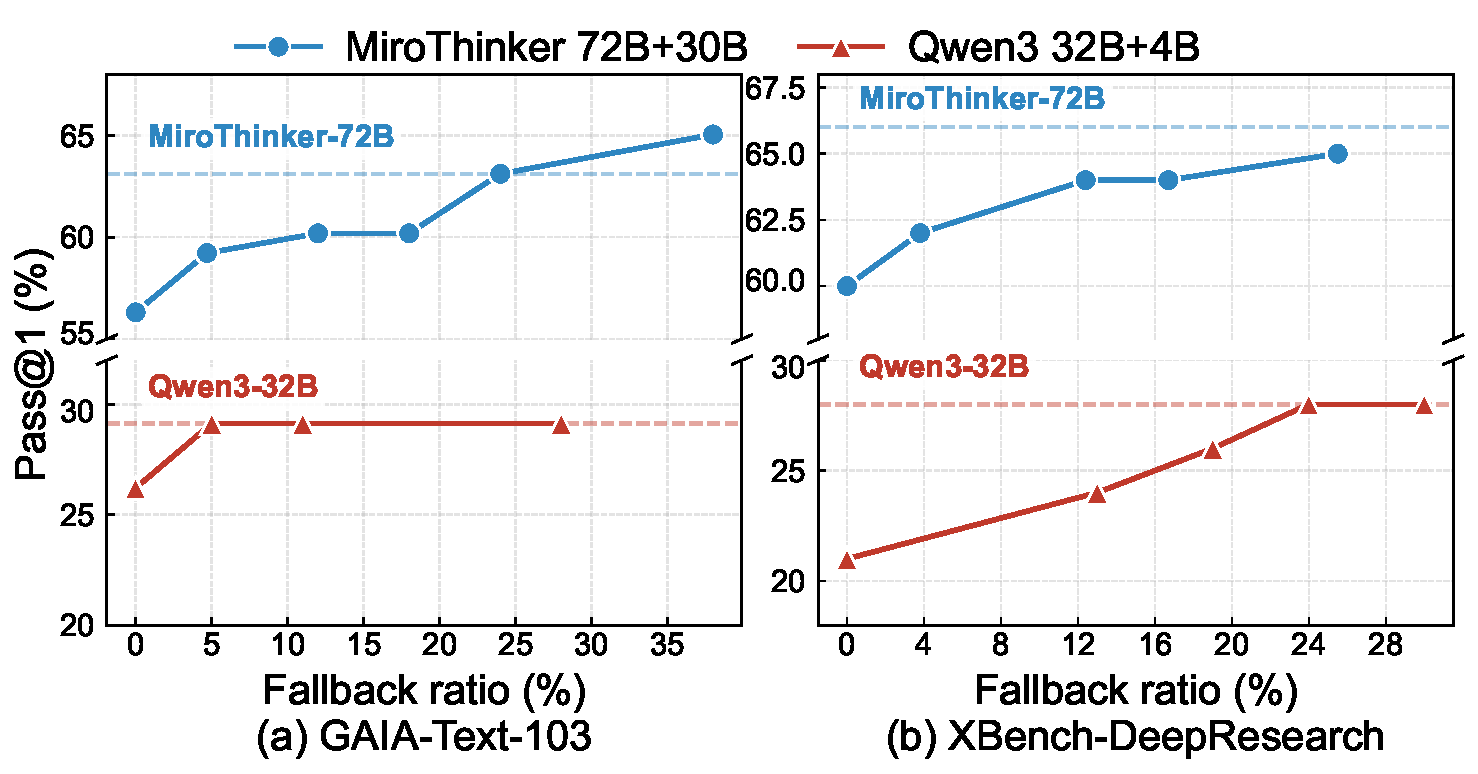
\includegraphics[width=\linewidth]{figs/threshold.pdf}
    \caption{Accuracy (pass@1) as a function of the reasoning intervention rate under a fixed drafting policy.}
    \label{fig:fallback_ratio}
\end{figure}

We study how accuracy changes with the frequency of the large model intervention. With a fixed speculator, we vary the verifier threshold, which indirectly controls the intervention rate. Accuracy increases as the intervention rate rises and then saturates. In practice, we observe that an intervention rate of about \textbf{20\% to 30\%} already reaches accuracy comparable to the base model, while retaining most of the latency benefit of heterogeneous speculation.

This trend is consistent across model families and datasets, with minor shifts in the saturation point. While tighter thresholds further improve accuracy, the returns diminish once the rate reaches the low-to-mid twenties. We therefore tune the threshold to target an intervention rate near 20\%, recovering near-base accuracy without sacrificing the efficiency benefits of sparse large-model reasoning.

\section{Conclusion}
% We presented \method{}, an efficient framework that accelerates deep research agents via \emph{heterogeneous action speculation}.
% Our key insight is that actions in deep research exhibit non-uniform uncertainty: Search often requires deliberative reasoning, while Visit is frequently more deterministic and can be executed without explicit reasoning.
% Leveraging this asymmetry, \method{} combines action-specific draft policies with semantic verification to enable reliable speculative execution while removing large-model reasoning from the critical path.
% Experiments across multiple benchmarks demonstrate that \method{} substantially reduces latency while preserving strong task success rates, highlighting the importance of action-aware speculation for scalable agentic systems.

We introduce \method{}, an efficient framework that accelerates deep research agents through heterogeneous action speculation.
Our key insight is that actions exhibit different uncertainty levels: Search often requires deliberative reasoning, whereas Visit is typically more deterministic and can be executed without reasoning.
Exploiting this asymmetry, \method{} integrates action-specific draft policies with semantic verification to enable reliable speculative execution while removing large-model reasoning from the critical path.
Experiments across multiple benchmarks show that \method{} significantly reduces latency while maintaining strong task success rates, highlighting the importance of action-aware speculation for scalable agentic systems.


\section*{Impact Statement}
This paper presents work whose goal is to advance the field of Machine Learning. There are many potential societal consequences of our work, none which we feel must be specifically highlighted here.

\newpage
\bibliography{example_paper}
\bibliographystyle{icml2026}

%%%%%%%%%%%%%%%%%%%%%%%%%%%%%%%%%%%%%%%%%%%%%%%%%%%%%%%%%%%%%%%%%%%%%%%%%%%%%%%
%%%%%%%%%%%%%%%%%%%%%%%%%%%%%%%%%%%%%%%%%%%%%%%%%%%%%%%%%%%%%%%%%%%%%%%%%%%%%%%
% APPENDIX
%%%%%%%%%%%%%%%%%%%%%%%%%%%%%%%%%%%%%%%%%%%%%%%%%%%%%%%%%%%%%%%%%%%%%%%%%%%%%%%
%%%%%%%%%%%%%%%%%%%%%%%%%%%%%%%%%%%%%%%%%%%%%%%%%%%%%%%%%%%%%%%%%%%%%%%%%%%%%%%
\newpage
\appendix
\onecolumn

\section{Verifier Prompt and Additional Analysis}
\label{app:verifier}

\subsection{Verifier Prompt Template}
\label{app:verifier_prompt}

Given the current state $s_t$ and a draft output consisting of an optional reasoning trace $z_t$ and a candidate action $a_t$, we query the large model as a critic to output a binary judgment (\texttt{Yes} or \texttt{No}).
The critic is instructed to jointly assess (i) whether the trajectory is making new progress toward the user goal and (ii) whether the proposed action is grounded and useful.
When the draft pathway skips explicit reasoning, we set $z_t=\emptyset$.
The exact prompt used for the critic is shown below.

\begin{quote}
\small
\noindent\textbf{[SYSTEM: TRAJECTORY AUDIT]}\\
Review the recent steps (context). Is the agent making \textbf{NEW PROGRESS}?\\[0.3em]
\noindent\textbf{REJECT ("No") if:}
\begin{enumerate}
    \item \textbf{Stagnation}: Repeating similar queries or visiting same URLs (Looping).
    \item \textbf{Ungrounded Answer}: The Final Answer is NOT supported by the \textit{retrieved search results}.
    \item \textbf{Lazy/Drift}: Queries are nested, vague, or irrelevant to User's Goal.
\end{enumerate}
\noindent Verdict: Is the trajectory HEALTHY and PROGRESSING?\\
Answer only "Yes" or "No".
\end{quote}

\subsection{Verifier Score Distributions}
\label{app:verifier_scores}

To further validate that the verifier score provides a meaningful signal, we analyze the score distributions on complete trajectories.
Specifically, we apply two full-size critics, MiroThinker-72B and Qwen3-32B, to evaluate step-level draft outputs produced by MiroThinker-8B and Qwen3-4B, respectively.
We report two aggregated statistics per trajectory: the mean score across all steps (\texttt{Mean}) and the 25th percentile score (\texttt{p25}), where \texttt{p25} emphasizes low-confidence segments within a trajectory.

\begin{figure}[H]
    \centering
    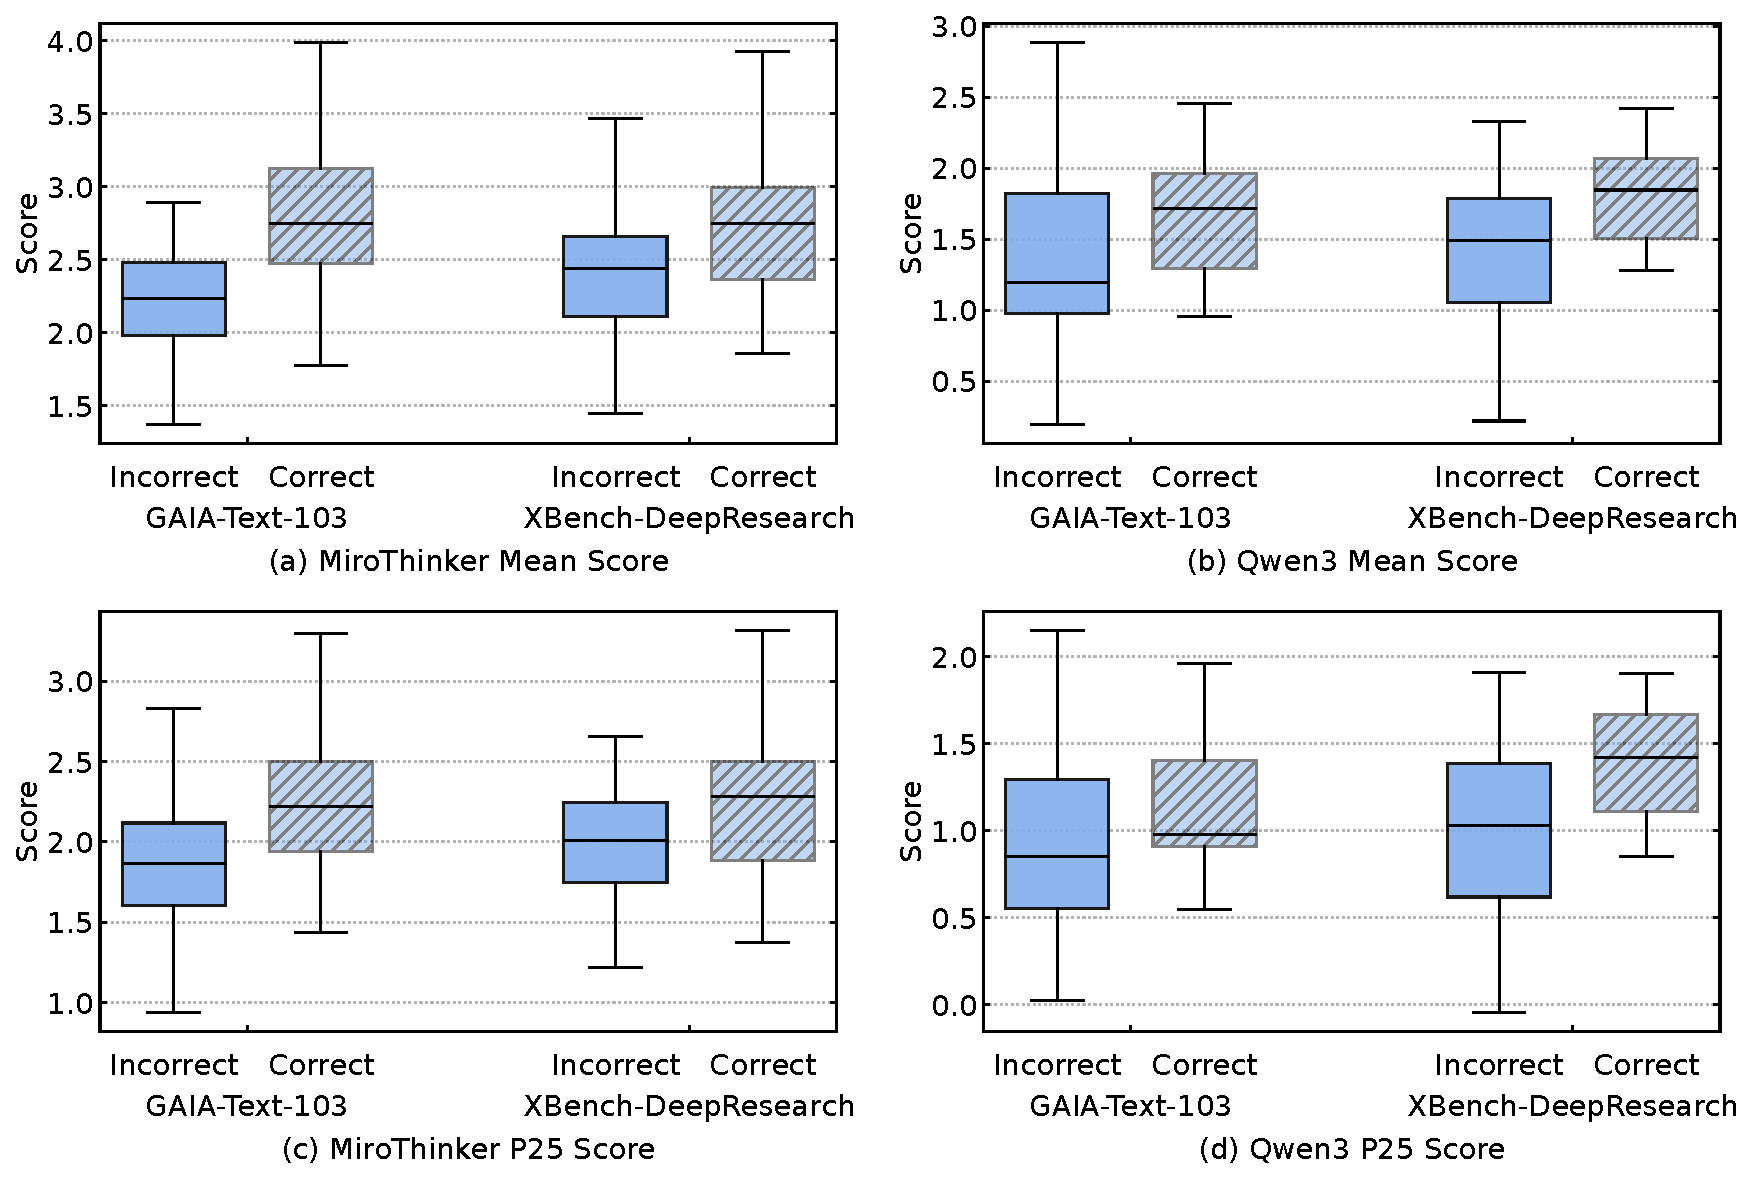
\includegraphics[width=0.8\linewidth]{figs/score.pdf}
    \caption{Verifier score distributions on GAIA and XBench-DeepResearch.
    We report trajectory-level aggregated verifier scores for (a) MiroThinker mean score, (b) Qwen mean score,
    (c) MiroThinker p25 score, and (d) Qwen p25 score.
    Correct trajectories consistently receive higher scores than incorrect ones, suggesting that the verifier provides a useful reliability signal.}
    \label{fig:verifier_score_dist}
\end{figure}

Figure~\ref{fig:verifier_score_dist} shows the score distributions on GAIA and XBench-DeepResearch, grouped by whether the final answer is correct.
Across both datasets and both model families, correct trajectories consistently exhibit higher verifier scores than incorrect ones under both \texttt{Mean} and \texttt{p25}.
This indicates that the verifier score correlates with end-to-end task success, supporting its use as a lightweight reliability signal for controlling speculative execution.




\end{document}

% This document was modified from the file originally made available by
% Pat Langley and Andrea Danyluk for ICML-2K. This version was created
% by Iain Murray in 2018, and modified by Alexandre Bouchard in
% 2019 and 2021 and by Csaba Szepesvari, Gang Niu and Sivan Sabato in 2022.
% Modified again in 2023 and 2024 by Sivan Sabato and Jonathan Scarlett.
% Previous contributors include Dan Roy, Lise Getoor and Tobias
% Scheffer, which was slightly modified from the 2010 version by
% Thorsten Joachims & Johannes Fuernkranz, slightly modified from the
% 2009 version by Kiri Wagstaff and Sam Roweis's 2008 version, which is
% slightly modified from Prasad Tadepalli's 2007 version which is a
% lightly changed version of the previous year's version by Andrew
% Moore, which was in turn edited from those of Kristian Kersting and
% Codrina Lauth. Alex Smola contributed to the algorithmic style files.
